You have $\nballs$ balls, and want to randomly distribute them among $\nbins$ different bins. Why? That's a pretty good question: basically, and you'll have to believe me for now, this rather strange scenario (and its many variants) capture a lot of actual interesting or well-motivated problems.\marginnote{We'll get back to those.}

The things we might care about are (1)~the \emph{maximum load} of the bins, that is, what's the maximum number of balls any given bin contains once we've distributed them; (2)~the \emph{coverage}, that is, how many bins are non-empty; and (3)~the \emph{collisions}, that is, how many pairs of distinct balls share the same bin.

The simplest thing we can do is throwing our $\nballs$ into the $\nbins$ independently and uniformly at random. Let's see how that goes.

\section{Collisions}
One of the most basic things we can ask is whether the $\nballs$ balls will all fall into their own personal bin, that is, if there's going to be at least one bin containing more than one ball. \emph{What's the probability to get at least one collision?}

\paragraph{Interlude:} \emph{run the Birthday Paradox experiment in the classroom. Discuss assumptions (uniformity), etc.}

\begin{theorem}[Birthday Paradox]
If you gather 23 people in a room, then with probability 50\% there will be two sharing a birthday.
\end{theorem}

To prove that, we'll tackle the more general question, for arbitrary $\nballs$ and $\nbins$, of finding what the probability $p_{\nballs, \nbins}$ of having at least one collision is: the birthday paradox is for $\nbins=366$, because, of course, 2024 is a leap year\marginnote{That might change in 2025...}, and asks to check that $p_{23,366} \geq 1/2$. Now, the result has to depend on the relation between $\nballs$ and $\nbins$: if $\nballs \geq \nbins + 1$, then that probability is exactly one,\marginnote{Do you see why? Prove it (Pigeonhole).} while if $\nbins \gg \nballs$ this should be less likely.

\begin{theorem}
    \label{theo:collisions:pnm}
    The probability $p_{\nballs, \nbins}$ to get at least one collision is equal to
    \begin{equation}
        \label{eq:collisions:pnm}
        p_{\nballs, \nbins} = 1 - \frac{\nbins!}{\nbins^{\nballs}(\nbins-\nballs)!} = 1 - \frac{\nballs!}{\nbins^{\nballs}} \binom{\nbins}{\nballs}
    \end{equation}
    In particular, for $\nballs = 23$ and $\nbins=366$, this is...?\marginnote{Check it: $p_{22,366} \approx 0.475$, while $p_{23,366} \approx 0.506$.}
\end{theorem}
\begin{proof}
    \begin{align*}
    1-p_{\nballs, \nbins} &= \frac{\nbins}{\nbins}\cdot\frac{\nbins-1}{\nbins}\cdot \frac{\nbins-2}{\nbins}\cdots \frac{\nbins-\nballs+1}{\nbins}
    = \frac{1}{\nbins^{\nballs}}\prod_{\ell=0}^{\nballs-1} (\nbins-\ell) \\
    &= \frac{\nbins!}{\nbins^{\nballs}(\nbins-\nballs)!} 
    \end{align*}
\end{proof}
\begin{figure}[htbp]
    \centering
    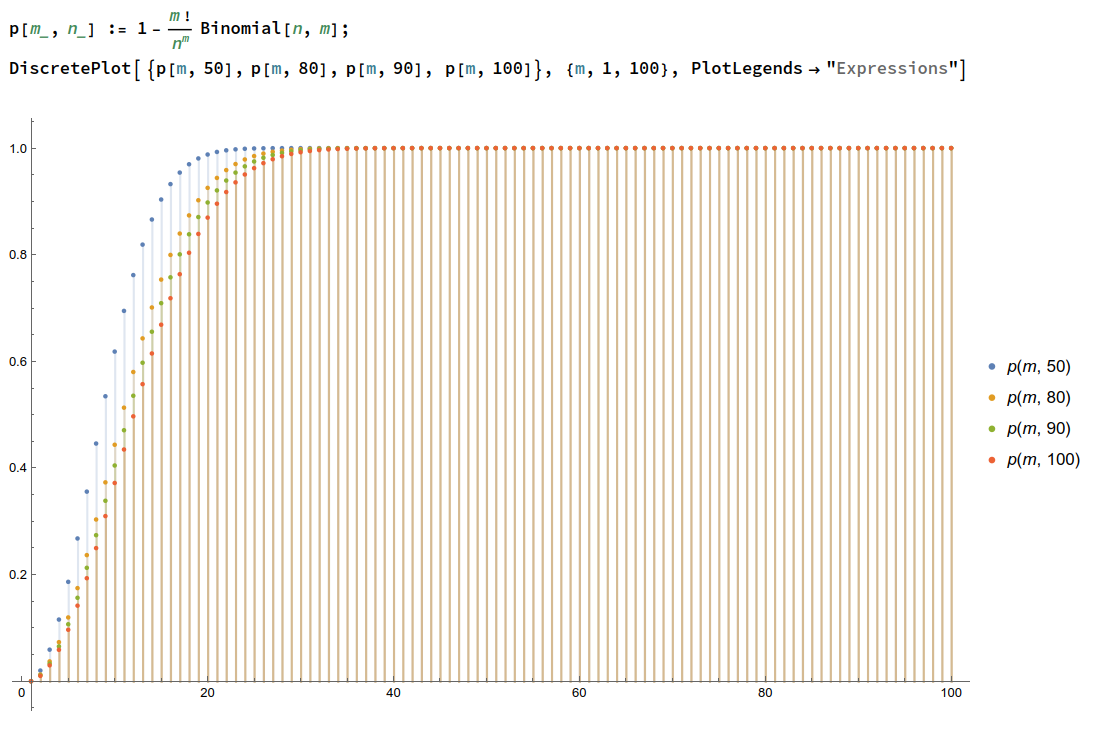
\includegraphics[width=1.0\textwidth]{figures/fig-collisions-nm.png}
    \caption{The quantity $p_{\nballs, \nbins}$ from~\cref{eq:collisions:pnm}, plotted here as a function of $\nballs$ for various choices of $\nbins$.}
    \label{fig:collisions:nm}
\end{figure}

Looking at the graph above, it looks like we approach a very high probability of getting a collision \emph{way} before $\nballs = \Theta(\nbins)$. Any guess at what $\nballs$ should be to, say, have probability at least $50\%$ of a collision? Should it be
\begin{itemize}
    \item $\Theta(\log\nbins)$?
    \item $\Theta(\sqrt{\nbins})$?
    \item $\Theta\Paren{\frac{\nbins}{\log\nbins}}$?
    \item Something else?
\end{itemize}
And \emph{why}?

\paragraph{The worst approach: rabbit-out-of-a-hat, no intuition given.} Take $\nballs = c\cdot\sqrt{\nbins}$ for some fixed constant $c>0$. Plugging this in the expression $p_{\nballs,\nbins}$ obtained in~\cref{theo:collisions:pnm}, we get
\begin{align*}
1 - p_{\nballs,\nbins} = \frac{\nbins!}{\nbins^{\nballs}(\nbins-\nballs)!}
&\operatorname*{\sim}_{\nbins\to\infty} 
\frac{1}{\nbins^{\nballs}}\cdot \frac{\sqrt{2\pi \nbins} \Paren{\frac{\nbins}{e}}^{\nbins}}{\sqrt{2\pi(\nbins-\nballs)}\Paren{\frac{\nbins-\nballs}{e}}^{\nbins-\nballs}} \tag{Stirling} \\
&= \frac{1}{\sqrt{1-\frac{\nballs}{\nbins}}} \frac{ \nbins^{\nbins-\nballs}}{\Paren{\nbins-\nballs}^{\nbins-\nballs} e^{\nballs}} \tag{``Massaging''}\\
&= \frac{1}{\sqrt{1-\frac{\nballs}{\nbins}}} \frac{1}{\Paren{1-\frac{\nballs}{\nbins}}^{\nbins-\nballs} e^{\nballs}} \\
&= \frac{1}{\sqrt{1-\frac{\nballs}{\nbins}}} \frac{1}{\Paren{1-\frac{\nballs}{\nbins}}^{\nbins} e^{\nballs}} \cdot \Paren{1-\frac{\nballs}{\nbins}}^{\nballs} \\
&= \frac{1}{\sqrt{1-\frac{c}{\sqrt{\nbins}}}} \frac{1}{\Paren{\Paren{1-\frac{c}{\sqrt{\nbins}}}^{\sqrt{\nbins}} e^{c}}^{\sqrt{\nbins}}} \cdot \Paren{1-\frac{c}{\sqrt{\nbins}}}^{c\sqrt{\nbins}} \tag{Finally!}
\end{align*}
the last line using our choice of $\nballs$. From there, ``all'' that remains to check is that $\lim_{\nbins\to\infty} \sqrt{1-\frac{c}{\sqrt{\nbins}}} = 1$ (easy), that 
\[
\lim_{\nbins\to\infty} \Paren{\Paren{1-\frac{c}{\sqrt{\nbins}}}^{\sqrt{\nbins}} e^{c}}^{\sqrt{\nbins}} = e^{-c^2/2}
\] (less easy)\marginnote{Do it!}, and that
\[
\lim_{\nbins\to\infty} \Paren{1-\frac{c}{\sqrt{\nbins}}}^{c\sqrt{\nbins}} = e^{-c^2}
\]
(not too hard?) to conclude that
\begin{align*}
1 - p_{c\sqrt{\nbins},\nbins} 
&\operatorname*{\sim}_{\nbins\to\infty} 1\cdot \frac{1}{e^{-c^2/2}} \cdot e^{-c^2} = e^{-c^2/2} 
\end{align*}
or, equivalently,
\begin{align*}
p_{c\sqrt{\nbins},\nbins} 
= 1 - e^{-c^2/2} +o(1)
\end{align*}
This shows that the probability to get a collision becomes constant for $\nballs = \Theta(\sqrt{\nbins})$.
Now, that's nice, but you may ask yourself, \emph{``Well, how did I get here?''}

\paragraph{Let's take a step back.} So we throw $\nballs$ balls into $\nbins$ bins. Let's start with the simplest case possible: let's throw \emph{two} balls into $\nbins$. What's the probability that they end up in the same bin?\marginnote{Don't look immediately! Think about it first.}\clearpage

The first ball falls into a given bin, say the $i$-th. Then to get a collision the second ball has to be thrown into the same bin $i$, which happens with probability $1/\nbins$. So $p_{2,\nbins} = 1/\nbins$. A more verbose way to derive it is as follows: let $\red{X_1}, \blue{X_2}$ denote the indices of the bins $\bin$ for the first $\balla$ and second $\ballb$ ball, respectively. These are independent r.v.'s, uniformly distributed in $[\nbins]$, so
\begin{align}
p_{2,\nbins} &= \probaOf{\red{X_1}=\blue{X_2}} = \sum_{k=1}^{\nbins} \probaOf{\red{X_1}=k, \blue{X_2}=k} \notag\\
&= \sum_{k=1}^{\nbins} \probaOf{\red{X_1}=k}\cdot\probaOf{\blue{X_2}=k} \notag\\
&= \sum_{k=1}^{\nbins} \frac{1}{\nbins}\cdot\frac{1}{\nbins} = \frac{\nbins}{\nbins^2} = \frac{1}{\nbins} \,,
\end{align}
``as foretold.''

Back to the general $\nballs$ balls case. The above tells us that for every pair of balls, the probability to get a collision (ignoring all other balls) is $1/\nbins$. How many distinct pairs of balls do we have? Well, $\binom{\nballs}{2}$. So what's the \emph{expected} number of collisions $c(\nballs,\nbins)$?
\begin{align}
   c(\nballs,\nbins) 
   &= \expect{\sum_{(\red{i},\blue{j})\text{ pair}} \indic{\red{X_i} = \blue{X_j}} }\notag\\
   &= \sum_{(\red{i},\blue{j})\text{ pair}} \expect{\indic{\red{X_i} = \blue{X_j}} }\notag\\
   &= \sum_{(\red{i},\blue{j})\text{ pair}} \probaOf{\red{X_i} = \blue{X_j}} \notag\\
   &= \sum_{(\red{i},\blue{j})\text{ pair}} \frac{1}{\nbins} \notag\\
   &= \binom{\nballs}{2}\cdot\frac{1}{\nbins} \label{eq:expect:collisions}
\end{align}
where we used linearity of expectation, and our previous computation for the $\nballs=2$ case. This means that the expected number of collisions grows (roughly) as $\frac{\nballs^2}{2\nbins}$. If we believe that the number of collisions does not deviate too pathologically from its expected value, this becomes constant when $\nballs = \bigTheta{\sqrt{\nbins}}$. So we should start expecting collisions when $\nballs = \bigTheta{\sqrt{\nbins}}$, which explains (in hindsight) the result we got before!

But can we easily prove this ``intuition''? We have the expectation $c(\nballs,\nbins)$ of the number of collisions, we want to show that number (let's call this random variable $C$) does not deviate too far from its expectation. The most basic tools we've seen for this are Markov and Chebyshev's inequalities: here, we'll have to use Chebyshev.\marginnote{Do you see why?} So we need to compute the variance of our random variable $C$:
\[
C = \sum_{(\red{i},\blue{j})\text{ pair}} \indic{\red{X_i} = \blue{X_j}}
\]
where as before \red{$X_i$} is the index of the bin \bin where the \red{$i$}-th ball \ball lands, and $\indic{\red{X_i} = \blue{X_j}}$ is the indicator of the event \emph{``ball $\red{i}$ and ball $\red{j}$ collide.''}
We \emph{would like} to write that the variance of the sum is the sum of the variances (``linearity of variance''), something like this
\begin{align*}
\var[C] 
&= \var\left[\sum_{(\red{i},\blue{j})\text{ pair}} \indic{\red{X_i} = \blue{X_j}}\right] 
\stackrel{?}{=} \sum_{(\red{i},\blue{j})\text{ pair}} \var\left[\indic{\red{X_i} = \blue{X_j}}\right] \\
\end{align*}
which \emph{would} make our life so much easier, since then, using the variance of an indicator random variable (Bernoulli), we'd get
\[
\var[C] = \binom{\nballs}{2}\frac{1}{\nbins}\Paren{1-\frac{1}{\nbins}}
\]
Unfortunately, \emph{variance is not linear}: we could write the above $\stackrel{?}{=}$ equality \emph{if} the indicator variables $\indic{\red{X_i} = \blue{X_j}}$ were independent (across $(\red{i},\blue{j})$): \emph{and this is not the case here}.\marginnote{Do you see why they are not independent?}

And yet, since we are showing the bin (for each ball) \emph{uniformly} at random, some magic happens, and somehow the above expression is still true.\marginnote{In the proof below, locate exactly where we use the fact that the bin is chosen uniformly.}
\begin{lemma}[Well, actually\dots \advancedstuff]
\label{lemma:variance:collisions}
We have 
\[
\var[C] = \binom{\nballs}{2}\frac{1}{\nbins}\Paren{1-\frac{1}{\nbins}}
\]
\end{lemma}
\begin{proof}
    Since $\var[C] = \bEE{C^2} - \bEE{C}^2$ and we already have computed $\bEE{C}$, we only are missing the first term:
    \begin{align*}
        \bEE{C^2} &= \bEE{\left(\sum_{(\red{i},\blue{j})\text{ pair}} \indic{\red{X_i} = \blue{X_j}}\right)^2} \\
        &= \bEE{\sum_{(\red{i},\blue{j})\text{ pair}}\sum_{(\orange{k},\green{\ell})\text{ pair}} \indic{\red{X_i} = \blue{X_j}}\indic{\orange{X_k} = \green{X_\ell}}} \\
        &= \sum_{(\red{i},\blue{j})\text{ pair}}\sum_{(\orange{k},\green{\ell})\text{ pair}} \bEE{\indic{\red{X_i} = \blue{X_j}}\indic{\orange{X_k} = \green{X_\ell}}} \\
    \end{align*}
    This is a little intimidating to compute, but we can make the following observations about the summands:
    \begin{itemize}
        \item if the two pairs $(\red{i},\blue{j})$, $(\orange{k},\green{\ell})$ are the same,\footnote{When we consider pairs here, we don't care about ordering, so $(i,j)=(j,i)$.} then $\indic{\red{X_i} = \blue{X_j}}\indic{\orange{X_k} = \green{X_\ell}} = \indic{\red{X_i} = \blue{X_j}}^2 = \indic{\red{X_i} = \blue{X_j}}$, so
        \[
            \bEE{\indic{\red{X_i} = \blue{X_j}}\indic{\orange{X_k} = \green{X_\ell}}} 
            = \bEE{\indic{\red{X_i} = \blue{X_j}}} 
            = \frac{1}{\nbins}\,.
        \]
        There are exactly $\binom{\nballs}{2}$ such summands.
        \item if the two pairs $(\red{i},\blue{j})$, $(\orange{k},\green{\ell})$ are disjoint, then $\indic{\red{X_i} = \blue{X_j}}$, $\indic{\orange{X_k} = \green{X_\ell}}$ are independent, and so
        \[
            \bEE{\indic{\red{X_i} = \blue{X_j}}\indic{\orange{X_k} = \green{X_\ell}}} 
            = \bEE{\indic{\red{X_i} = \blue{X_j}}} \bEE{\indic{\orange{X_k} = \green{X_\ell}}} 
            = \frac{1}{\nbins^2}\,.
        \]
        There are exactly $\binom{\nballs}{2}\binom{\nballs-2}{2}$ such summands.
        \item else, then the two pairs $(\red{i},\blue{j})$, $(\orange{k},\green{\ell})$ are neither disjoint nor equal, then $|\{\red{i},\blue{j},\orange{k},\green{\ell}\}|=3$. For any such summand, $\indic{\red{X_i} = \blue{X_j}}\indic{\orange{X_k} = \green{X_\ell}}$ is of the form $\indic{\red{X_i} = \blue{X_j} = \orange{X_k}}$, and so
        \begin{align*}
            \bEE{\indic{\red{X_i} = \blue{X_j}}\indic{\orange{X_k} = \green{X_\ell}}} 
            &= \bEE{\indic{\red{X_i} = \blue{X_j} = \orange{X_k}}} \\
            &= \sum_{b=1}^{\nbins} \probaOf{\red{X_i} = b,  \blue{X_j} = b, \orange{X_k} = b} \\
            &= \frac{\nbins}{\nbins^3}\\
            &= \frac{1}{\nbins^2}\,.
        \end{align*}
        There are exactly $2\cdot \binom{3}{2}\binom{\nballs}{3} = 6\binom{\nballs}{3}$ such summands.\marginnote{Can you see why? (If that's any consolation, I am terrible at combinatorics.)}
    \end{itemize}
    As a sanity check, we do have $\binom{\nballs}{2} + \binom{\nballs}{2}\binom{\nballs-2}{2} + 6\binom{\nballs}{3} = \binom{\nballs}{2}^2$, so we did not miss any summand in the above distinction of cases. We can then rewrite
    \begin{align*}
        \bEE{C^2} 
        &= \binom{\nballs}{2}\cdot \frac{1}{\nbins}
        + \binom{\nballs}{2}\binom{\nballs-2}{2}\cdot \frac{1}{\nbins^2}
        + 6\binom{\nballs}{3}\cdot \frac{1}{\nbins^2} \\
        &= \binom{\nballs}{2}\cdot \frac{1}{\nbins} + \binom{\nballs}{2}^2\cdot \frac{1}{\nbins^2} - \binom{\nballs}{2}\cdot \frac{1}{\nbins^2} \tag{Magic?} \\
        &= \binom{\nballs}{2}\cdot \frac{1}{\nbins}\Paren{1-\frac{1}{\nbins}} + \binom{\nballs}{2}^2\cdot \frac{1}{\nbins^2} 
    \end{align*}
    That's really encouraging, since the second term is exactly $\bEE{C}^2$, and the first is what we were hoping to get for the variance. And, indeed:
    \begin{align*}
        \var[C] &= \bEE{C^2} - \bEE{C}^2
        = \binom{\nballs}{2}\frac{1}{\nbins}\Paren{1-\frac{1}{\nbins}} + \binom{\nballs}{2}^2 \frac{1}{\nbins^2}  - \Paren{\binom{\nballs}{2} \frac{1}{\nbins}}^2 \\
        &= \binom{\nballs}{2} \frac{1}{\nbins}\Paren{1-\frac{1}{\nbins}}\,,
    \end{align*}
    concluding the proof.
\end{proof}
\begin{framed}
Here, we were lucky: somehow in the variance calculation some terms ``magically cancel out'' and we get the same expression as if things were independent. \emph{This is not usually the case!} But there are some `ways to handle things nonetheless. For instance:
\begin{itemize}
    \item If $X_1,\dots,X_n$ are \emph{negatively correlated}, then 
    \[
    \var[\sum_{i=1}^n X_i] \leq \sum_{i=1}^n \var[X_i]
    \]
    \item Since $\var[X] = \expect{X^2} - \expect{X}^2$, we can always write
    \[
    \var[X] \leq \expect{X^2}\,.
    \]
    Sometimes, it's good enough!
\end{itemize}  
\end{framed}\marginnote{There are also other ``fancier'' ways, such as the Efron--Stein inequality, but that's slightly out of scope. Check it out if interested!}  

Now we have the expectation (\cref{eq:expect:collisions}), we have the variance (\cref{lemma:variance:collisions}), and we have Chebyshev. For any $t>0$,
\[
\probaOf{|C - c(\nballs,\nbins)| \geq t} \leq \frac{\var[C]}{t^2} \leq \frac{c(\nballs,\nbins)}{t^2}
\]
Let's set $\nballs = \flr{3\sqrt{\nbins}}$, so that (using $\nbins \geq 2$)
\[
c(\nballs,\nbins) = \binom{\flr{3\sqrt{\nbins}}}{2}\cdot\frac{1}{\nbins} \geq 2
\]
(it's not immediate, but can be checked); and $t \eqdef c(\nballs,\nbins)$. We then have
\[
\probaOf{C=0} \leq \probaOf{|C - c(\nballs,\nbins)| \geq c(\nballs,\nbins)} \leq \frac{1}{c(\nballs,\nbins)} \leq \frac{1}{2}
\]
showing that \emph{we have at least a 50\% chance to get a collision as soon as $\nballs \geq \flr{3\sqrt{\nbins}}$.} And conversely, using this time Markov's inequality,\marginnote{This inequality, $\probaOf{X=0} \geq 1-\expect{X}$ for $X$ integer-valued, is sometimes referred to as the \emph{first moment method}.}
\[
\probaOf{C\neq 0} = \probaOf{C\geq 1}  \leq \expect{C} = c(\nballs,\nbins) \leq \frac{\nballs^2}{2\nbins}
\]
which is less than $50\%$ for $\nballs \leq \flr{\sqrt{\nbins}}$. To sum up, we proved, using Chebyshev's and Markov's inequalities:
\begin{theorem}
    The probability to get \emph{at least one collision} when throwing $\nballs$ independent and uniformly at random in $\nbins$ bins is less than $1/2$ when $\nballs \leq \flr{\sqrt{\nbins}}$, and at least $1/2$ as soon as $\nballs \geq \flr{\sqrt{3\nbins}}$.
\end{theorem}
\noindent confirming the empirical observations and (hopefully) gaining some intuition along the way.

\subsection{Applications}

\begin{itemize}
    \item Hashing, and hash functions
    \item Distribution testing (statistics)
    \item Lower bounds for other problems!
\end{itemize}

\section{Coverage}
Another very natural thing to ask is \emph{when each bin will have received at least one ball}. This is often referred to as the \emph{coupon collector} problem, a term coined a long time ago, when computer scientists were eating cereals for breakfast hoping to collect all of the coupons (cards) of a collection, one cereal box at a time.\marginnote{We will stick with the balls-and-bins scenario. But yes, gotta catch'em all!}

Obviously, since we are trying to hit at least each of $\nbins$ bins at least once, we need to throw at least $\nballs \geq \nbins$ balls. But is it enough?
\begin{framed}
    \noindent What is the expected number of balls $\green{M}(\nbins)$ one needs to throw before each of the $\nbins$ bins contains at least one of the $\nballs$ balls?
\end{framed}
To figure it out, we can start by trying to simulate the experiment.\marginnote{This code is definitely \emph{not} optimised!}
\begin{lstlisting}
import numpy as np
import random
def coverage(n):
    (m,ncovered) = (0,0)
    covered = np.zeros(n)
    while ncovered < n:
        draw = random.randint(1, n);
        if covered[draw-1] == 0:
            covered[draw-1] = 1
            ncovered += 1
        m += 1
    return m
\end{lstlisting}
\begin{lstlisting}
list_n = np.arange(10, 1001);
experiments_avg = np.zeros(np.size(list_n));
experiments_std = np.zeros(np.size(list_n));
for i in range(len(list_n)):
    coverages_trials = [coverage(list_n[i]) for _ in range(100)];
    experiments_avg[i] = np.mean(coverages_trials);
    experiments_std[i] = np.std(coverages_trials);
\end{lstlisting}
\begin{figure}[htbp]\centering
    \label{fig:coverage:1}
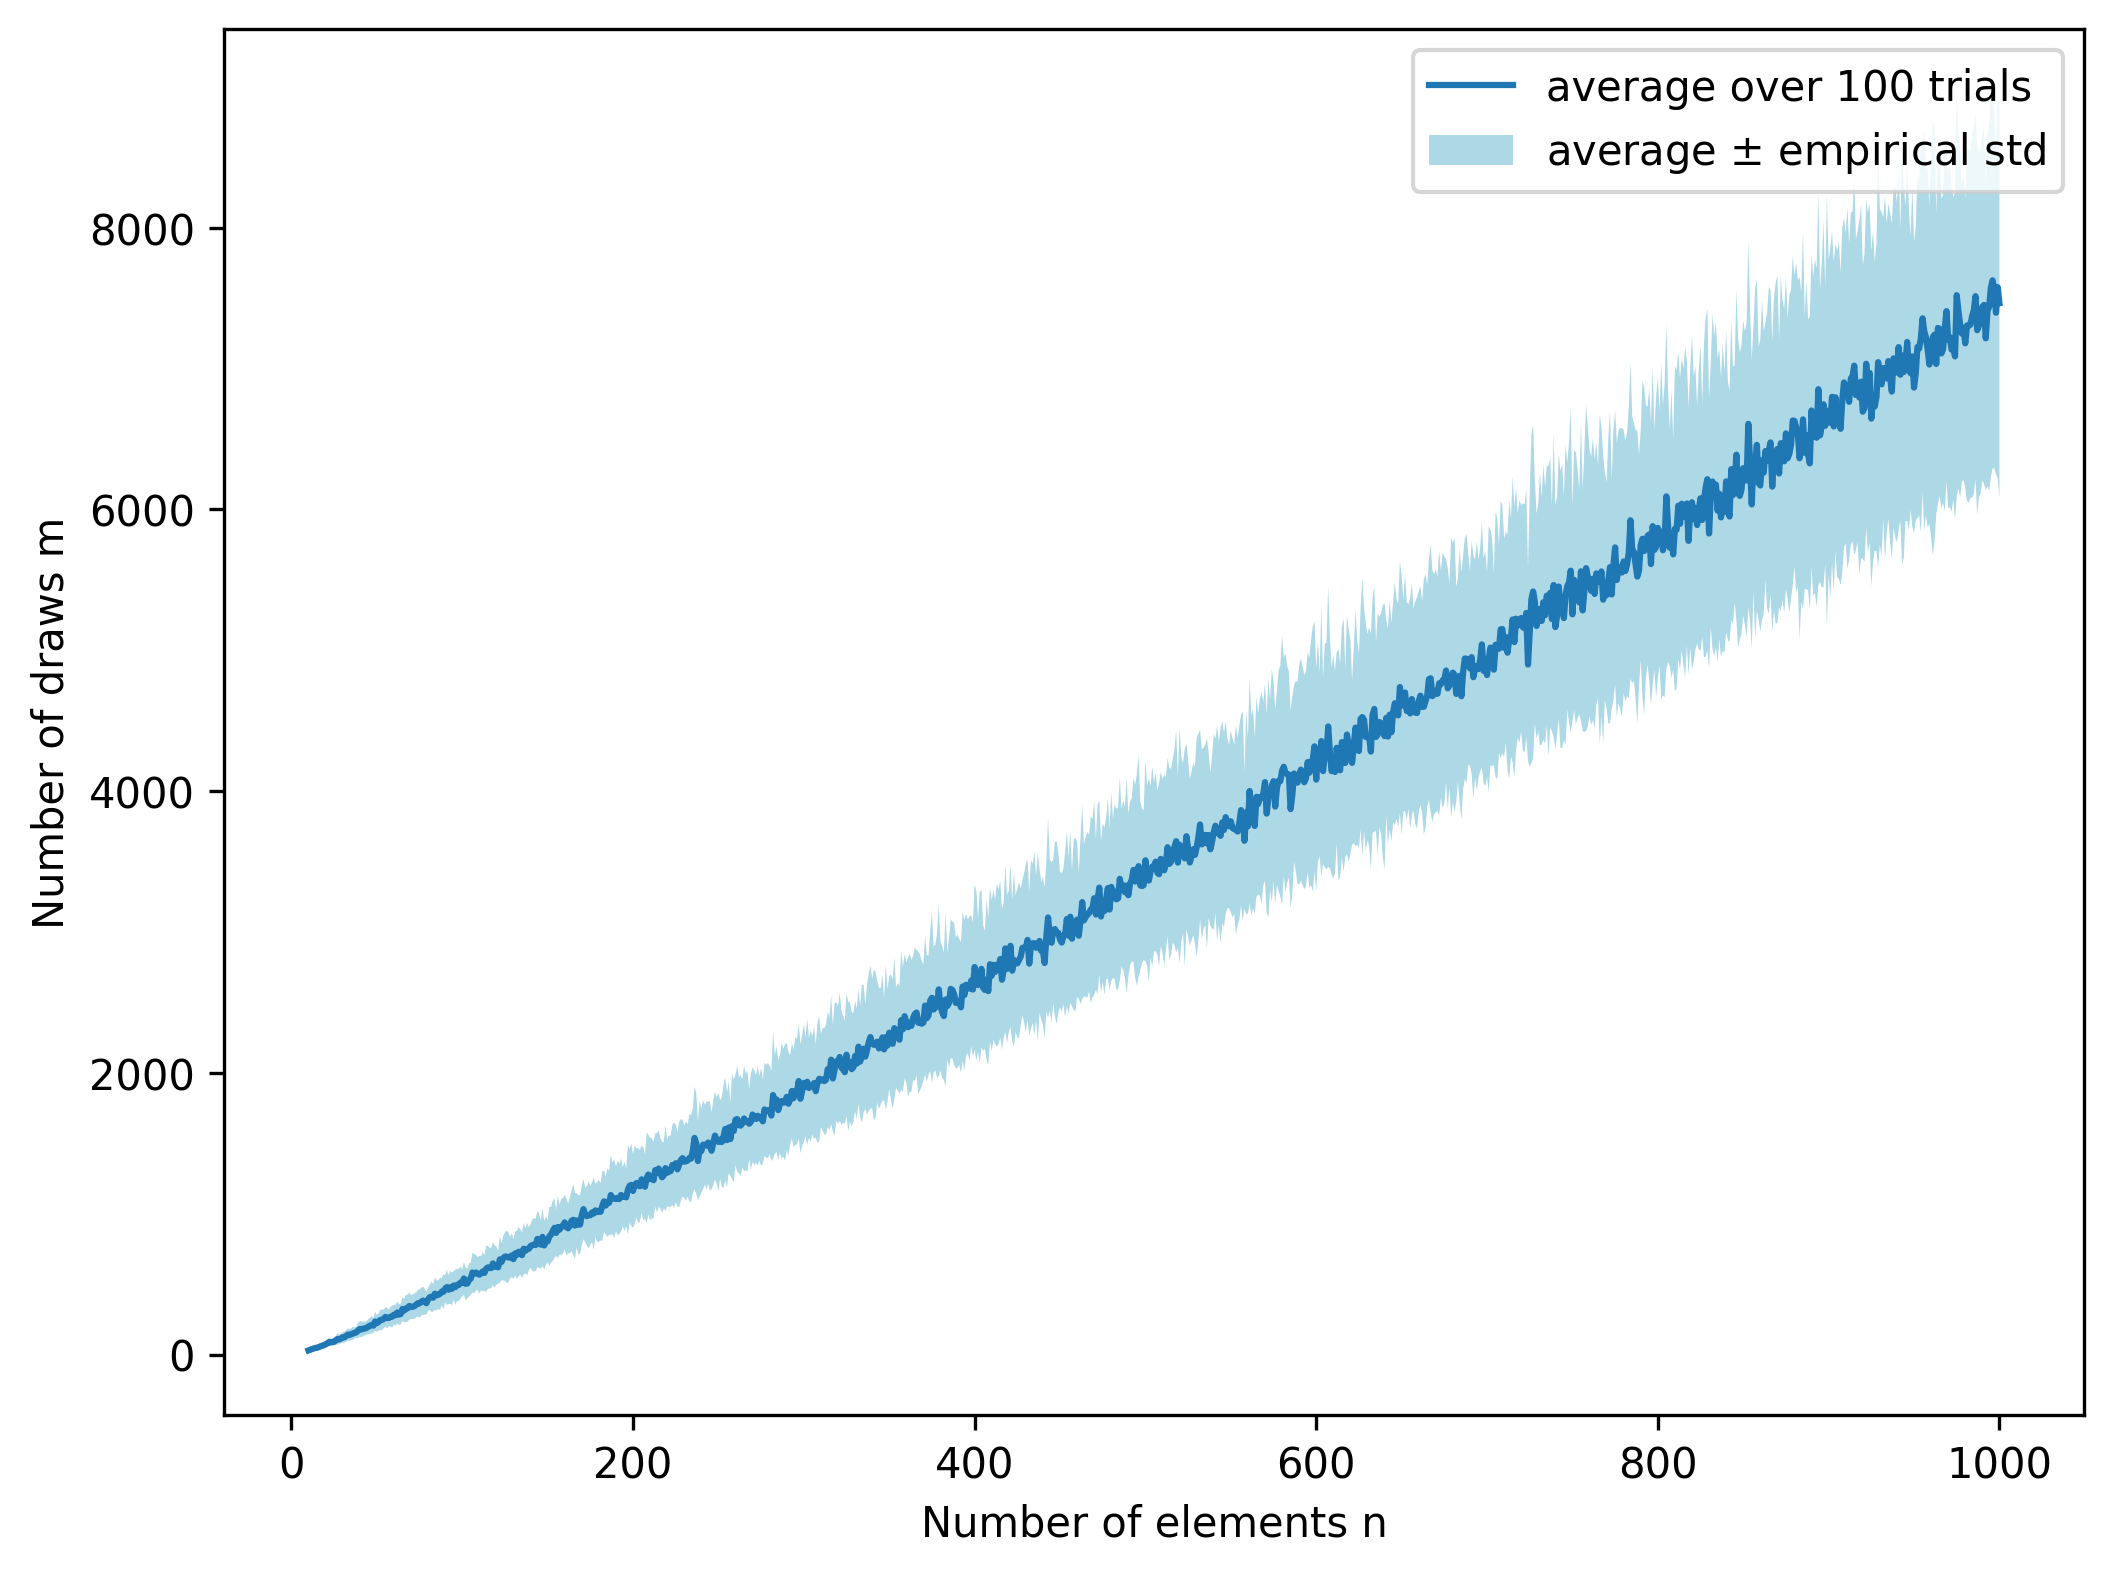
\includegraphics[width=0.9\textwidth]{figures/fig-coverage1.png}
\caption{Average (over 100 trials) of the number of balls thrown until all of the $\nbins$ bins contain at least one ball, as a function of $\nbins$. The range given by one empirical standard deviation is plotted alongside.}
\end{figure}

Looking at the graph above, we can see how the average number of balls to throw grows with $\nbins$. But what is it, quantitatively? How does $\green{M}(\nbins)$ behaves?
\begin{itemize}
    \item $\Theta(\nbins)$?
    \item $\Theta(\nbins\log\nbins)$?
    \item $\Theta(\nbins^{3/2})$?
    \item Something else?
\end{itemize}
And \emph{why}?

\paragraph{Some intuition.} Let's look at what happens when $\nballs=\nbins$: how many bins \emph{haven't} been hit by a balls when we have thrown $\nbins$ of them. The probability a fixed bin does not contain any ball is
\[
\Paren{1-\frac{1}{\nbins}}^{\nbins} \approx e^{-1}
\]
and so the expected number of bins with no balls, by linearity of expectation, is
\begin{equation}
    \label{eq:expected:empty:bins}
\expect{\text{empty bins after }\nbins\text{  balls}}=\sum_{i=1}^{\nbins} \probaOf{\substack{\text{bin $i$ empty}\\\text{ after }\nbins\text{  balls}}} =\nbins\cdot \Paren{1-\frac{1}{\nbins}}^{\nbins} \approx \frac{\nbins}{e}
\end{equation}
This means that after throwing $\nbins$ balls, we still have a constant fraction ($\approx 1/e$) of bins to still hit. Repeating the argument, if we throw $\nbins$ more balls, we expect to still have $\approx 1/e^2$ empty bins; $\nbins$ more balls, and the remaining fraction will be $\approx1/e^3$; etc. Each time we throw $\nbins$ more balls, we decrease (in expectation) the number of empty bins by a constant factor, so\dots{} to bring the expected number of empty bins to $<1$, we'll need to repeat that $\Theta(\log\nbins)$ times.\marginnote{Generalise~\cref{eq:expected:empty:bins} to $\nballs$ bins, to compute directly \[\expect{\text{empty bins after }\nballs\text{  balls}}\] and solve for $\nballs$ to get this expectation to be less than $1$, say $1/2$. Show you retrieve the $\Theta(\nbins\log\nbins)$.} This argument tells us that 
\[
\green{M}(\nbins) = \Theta(\log\nbins)\cdot \nbins = \Theta(\nbins\log\nbins)
\]
sounds reasonable. Can we prove it?

\begin{theorem}
    \label{theo:coupon:collector:expectation}
    We have 
    \[
    \green{M}(\nbins) = \nbins H_{\nbins}\,.
    \]
    where $H_{\nbins} = \sum_{k=1}^{\nbins} \frac{1}{k}$ is the $\nbins$-th Harmonic number.
\end{theorem}
\noindent Before proving this, recall the following fact:\marginnote{Prove the first-order term: $H_n = \Theta(n\log n)$.} % Tutorial
\begin{fact}
\label{fact:harmonic}
    The $n$-th Harmonic number satisfies
    \[
        H_n = \ln n + \gamma + O(1)\,,
    \]
    where $\ln$ is the natural logarithm and $\gamma\approx 0.5772$ is the Euler--Mascheroni constant.
\end{fact}
\begin{proof}[Proof~of~\cref{theo:coupon:collector:expectation}]
To establish this result, we will introduce some auxiliary random variables, so that we can reduce everything to the one good tool we have~--~linearity of expectation. For $1\leq i\leq \nbins$, denote by $T_i$ the number of balls needed, after hitting the $(i-1)$-th distinct bin so far, to hit a new one (the $i$-th bin). So for instance, $T_1=1$ (the first ball we throw by definition hits a new bin, and we had not hit any before), and $T_2$ is the number of balls we need to throw after that to get a ball in another bin than that first one. It's at least $1$, and, if we're unlucky and keep throwing balls into the very same bin, could be much more than that.

The total number of balls to throw before hitting all bins is then, by definition,
\[
T_1+T_2+\cdots+T_{\nbins}
\]
and so, by linearity of expectation,
\begin{equation}
    \label{expect:coverage:proofstep}
\green{M}(\nbins) = \expect{T_1+T_2+\cdots+T_{\nbins}}
= \sum_{i=1}^{\nbins} \expect{T_i}\,.
\end{equation}
It remains to get a handle on $\expect{T_i}$, for $i\geq 1$. We have seen that $T_1=1$ always, so $\expect{T_1}=1$; what about $i\geq 2$? Given that we have hit $i-1$ distinct bins already, the next ball we throw has a probability
\[
\frac{\nbins-(i-1)}{\nbins} = \frac{\nbins-i+1}{\nbins}
\]
to hit one of the remaining empty $\nbins-(i-1)$ bins, out of $\nbins$ total. We keep throwing balls, each with this probability of success, until we do hit an empty bin: so $T_i$ is a Geometric random variable\marginnote{See previous chapter.} with parameter $p_i \eqdef \frac{\nbins-i+1}{\nbins}$, and so its expectation is
\[
    \expect{T_i} = \frac{1}{p_i} = \frac{\nbins}{\nbins-i+1}\,.
\]
Plugging this in~\eqref{expect:coverage:proofstep} gives us
\[
\green{M}(\nbins) = \sum_{i=1}^{\nbins} \frac{\nbins}{\nbins-i+1}
= \sum_{j=1}^{\nbins} \frac{\nbins}{j}
= \nbins H_{\nbins}
\]
concluding the proof.
\end{proof}
Before going further, let us see how this identity we just proved compared to our empirical average:
\begin{figure}[htbp]\centering
    \label{fig:coverage:2}
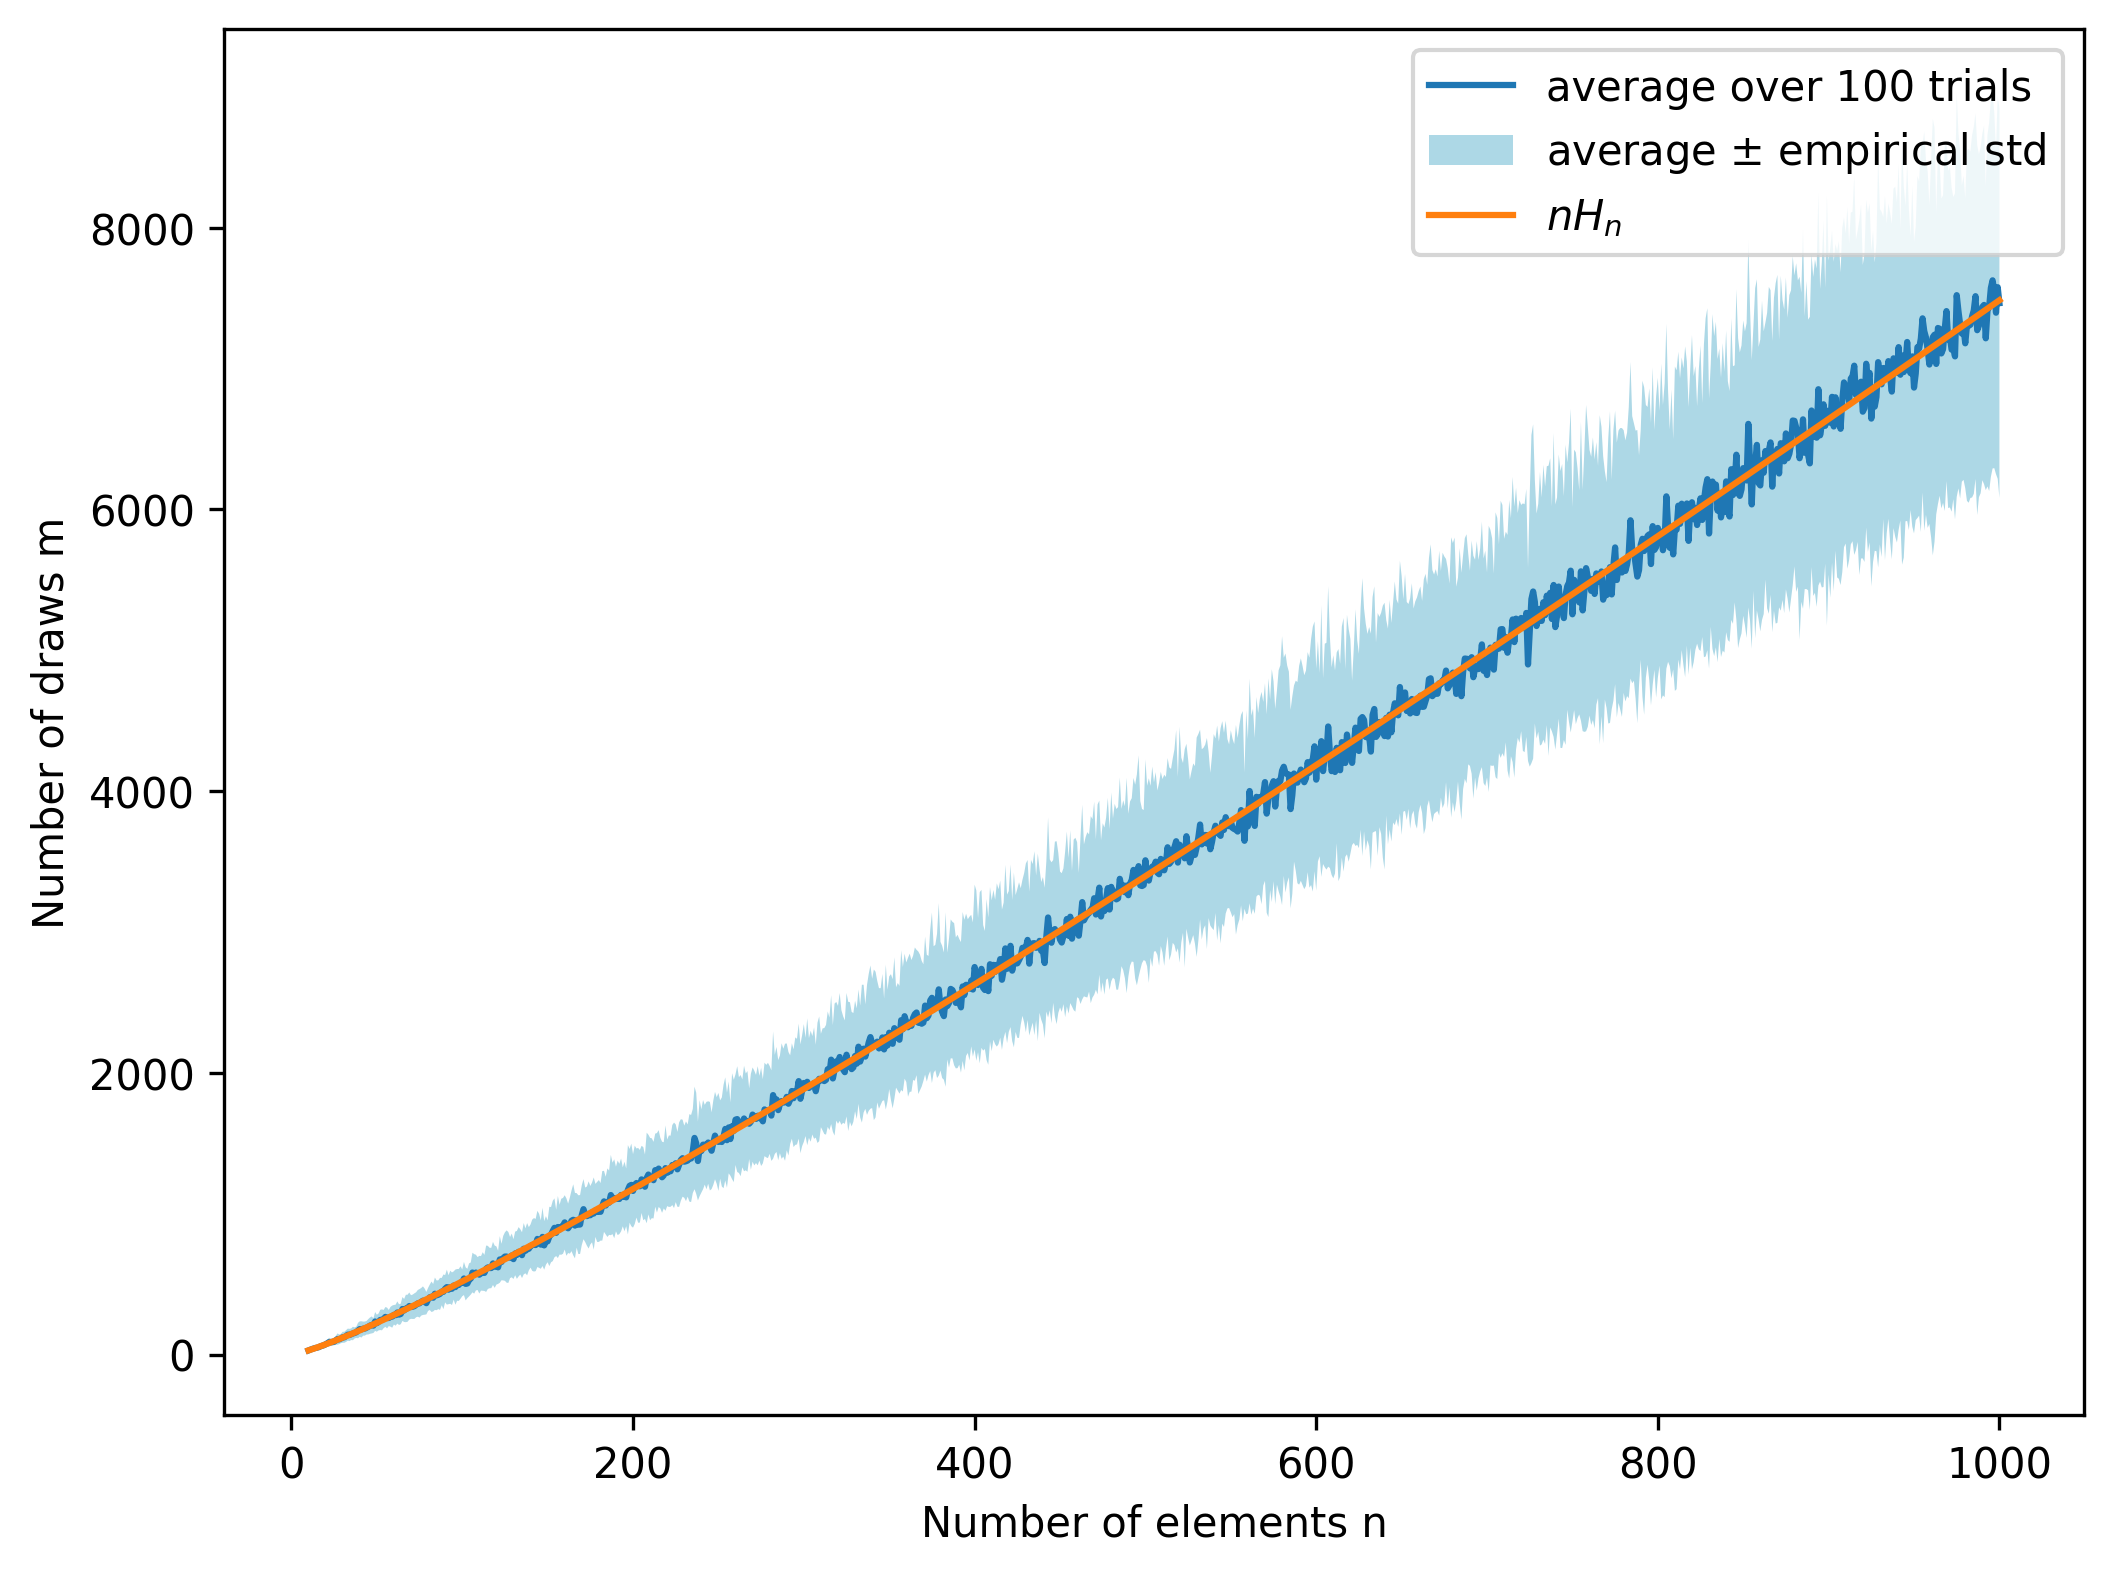
\includegraphics[width=0.9\textwidth]{figures/fig-coverage2.png}
\caption{Average (over 100 trials) of the number of balls thrown until all of the $\nbins$ bins contain at least one ball, as a function of $\nbins$, along with the theoretical value $\nbins H_{\nbins}$ shown in~\cref{theo:coupon:collector:expectation}. The range given by one empirical standard deviation is plotted alongside.}
\end{figure}

Not bad! That does it for the expectation\dots{} but the figure also hints the variance is not too bad, and the number of balls needed to hit all $\nbins$ looks quite concentrated around its expectation. To confirm this (in view of, if we wanted to, applying Chebyshev's inequality), can we also compute the variance?

The amazing thing is that not only we \emph{can}, it's also quite easy.
\begin{theorem}
    \label{theo:coupon:collector:variance}
    The variance of the number $\green{m}(\nbins)$ of bins needed to hit all $\nbins$ bins satisfies
    \[
    \var[\green{m}(\nbins)] \leq \frac{\pi^2}{6}\nbins^2\,.
    \]
\end{theorem}
\begin{proof}
    We start as in the proof of~\cref{theo:coupon:collector:expectation}, writing
    \[
        \green{m}(\nbins) = T_1+\dots+T_{\nbins}
    \]
    The crucial observation is that (suprinsingly?), \emph{the random variables $T_1,\dots,T_{\nbins}$ are independent.} Intuitively, this is because, once you have hit $i-1$ bins, the number of \emph{new} balls you need to cover the remaining $\nbins-(i-1)$ does not depend on how many balls you already threw: it only depends on $\nbins$ and $i$, and ``doesn't care about the past.''\marginnote{This is called the \href{https://en.wikipedia.org/wiki/Geometric_distribution\#General_properties}{memorylessness property} of the geometric distribution, but try to first convince yourself of this without giving it a label.}

    This is great, because computing the variance becomes immediate:
    \[
    \var[\green{m}(\nbins)]=\var[T_1+\dots+T_{\nbins}]
    = \sum_{i=1}^{\nbins} \var[T_i]
    \]
    and we already saw that $T_i \sim \operatorname{Geom}\Paren{p_i}$ with $p_i=\frac{\nbins-i+1}{\nbins}$, ``so'' its variance is \marginnote{Check it yourself: we don't lose much by ignoring the $-p_i$ term.}
    \[
    \var[T_i] = \frac{1-p_i}{p_i^2} \leq \frac{1}{p_i^2}= \frac{\nbins^2}{(\nbins-i+1)^2}
    \]
    and we get
    \[
    \var[\green{m}(\nbins)]
    \leq \nbins^2\cdot\sum_{i=1}^{\nbins} \frac{1}{(\nbins-i+1)^2}
    =\nbins^2\cdot\sum_{j=1}^{\nbins} \frac{1}{j^2}
    \leq \nbins^2\cdot \frac{\pi^2}{6}\,,
    \]
    the last inequality recalling that
    $\sum_{k=1}^{\infty}\frac{1}{k^2} = \frac{\pi^2}{6}$.
\end{proof}
We won't go through too much here, but for instance, by Chebyshev's inequality, this means that
\begin{equation}
    \green{m}(\nbins) = \nbins H_{\nbins} \pm O(\nbins)
\end{equation}
with probability at least $0.99$; combining this with~\cref{fact:harmonic}, similarly,
\begin{equation}
    \green{m}(\nbins) = \nbins \ln \nbins \pm O(\nbins)
\end{equation}
with probability at least $0.99$ (with a different constant in the $O(\cdot)$).

To conclude this part\dots{} how did we do with this variance bound? Well, let us see the empirical simulation again, adding them to the mix:
\begin{figure}[htbp]\centering
    \label{fig:coverage:3}
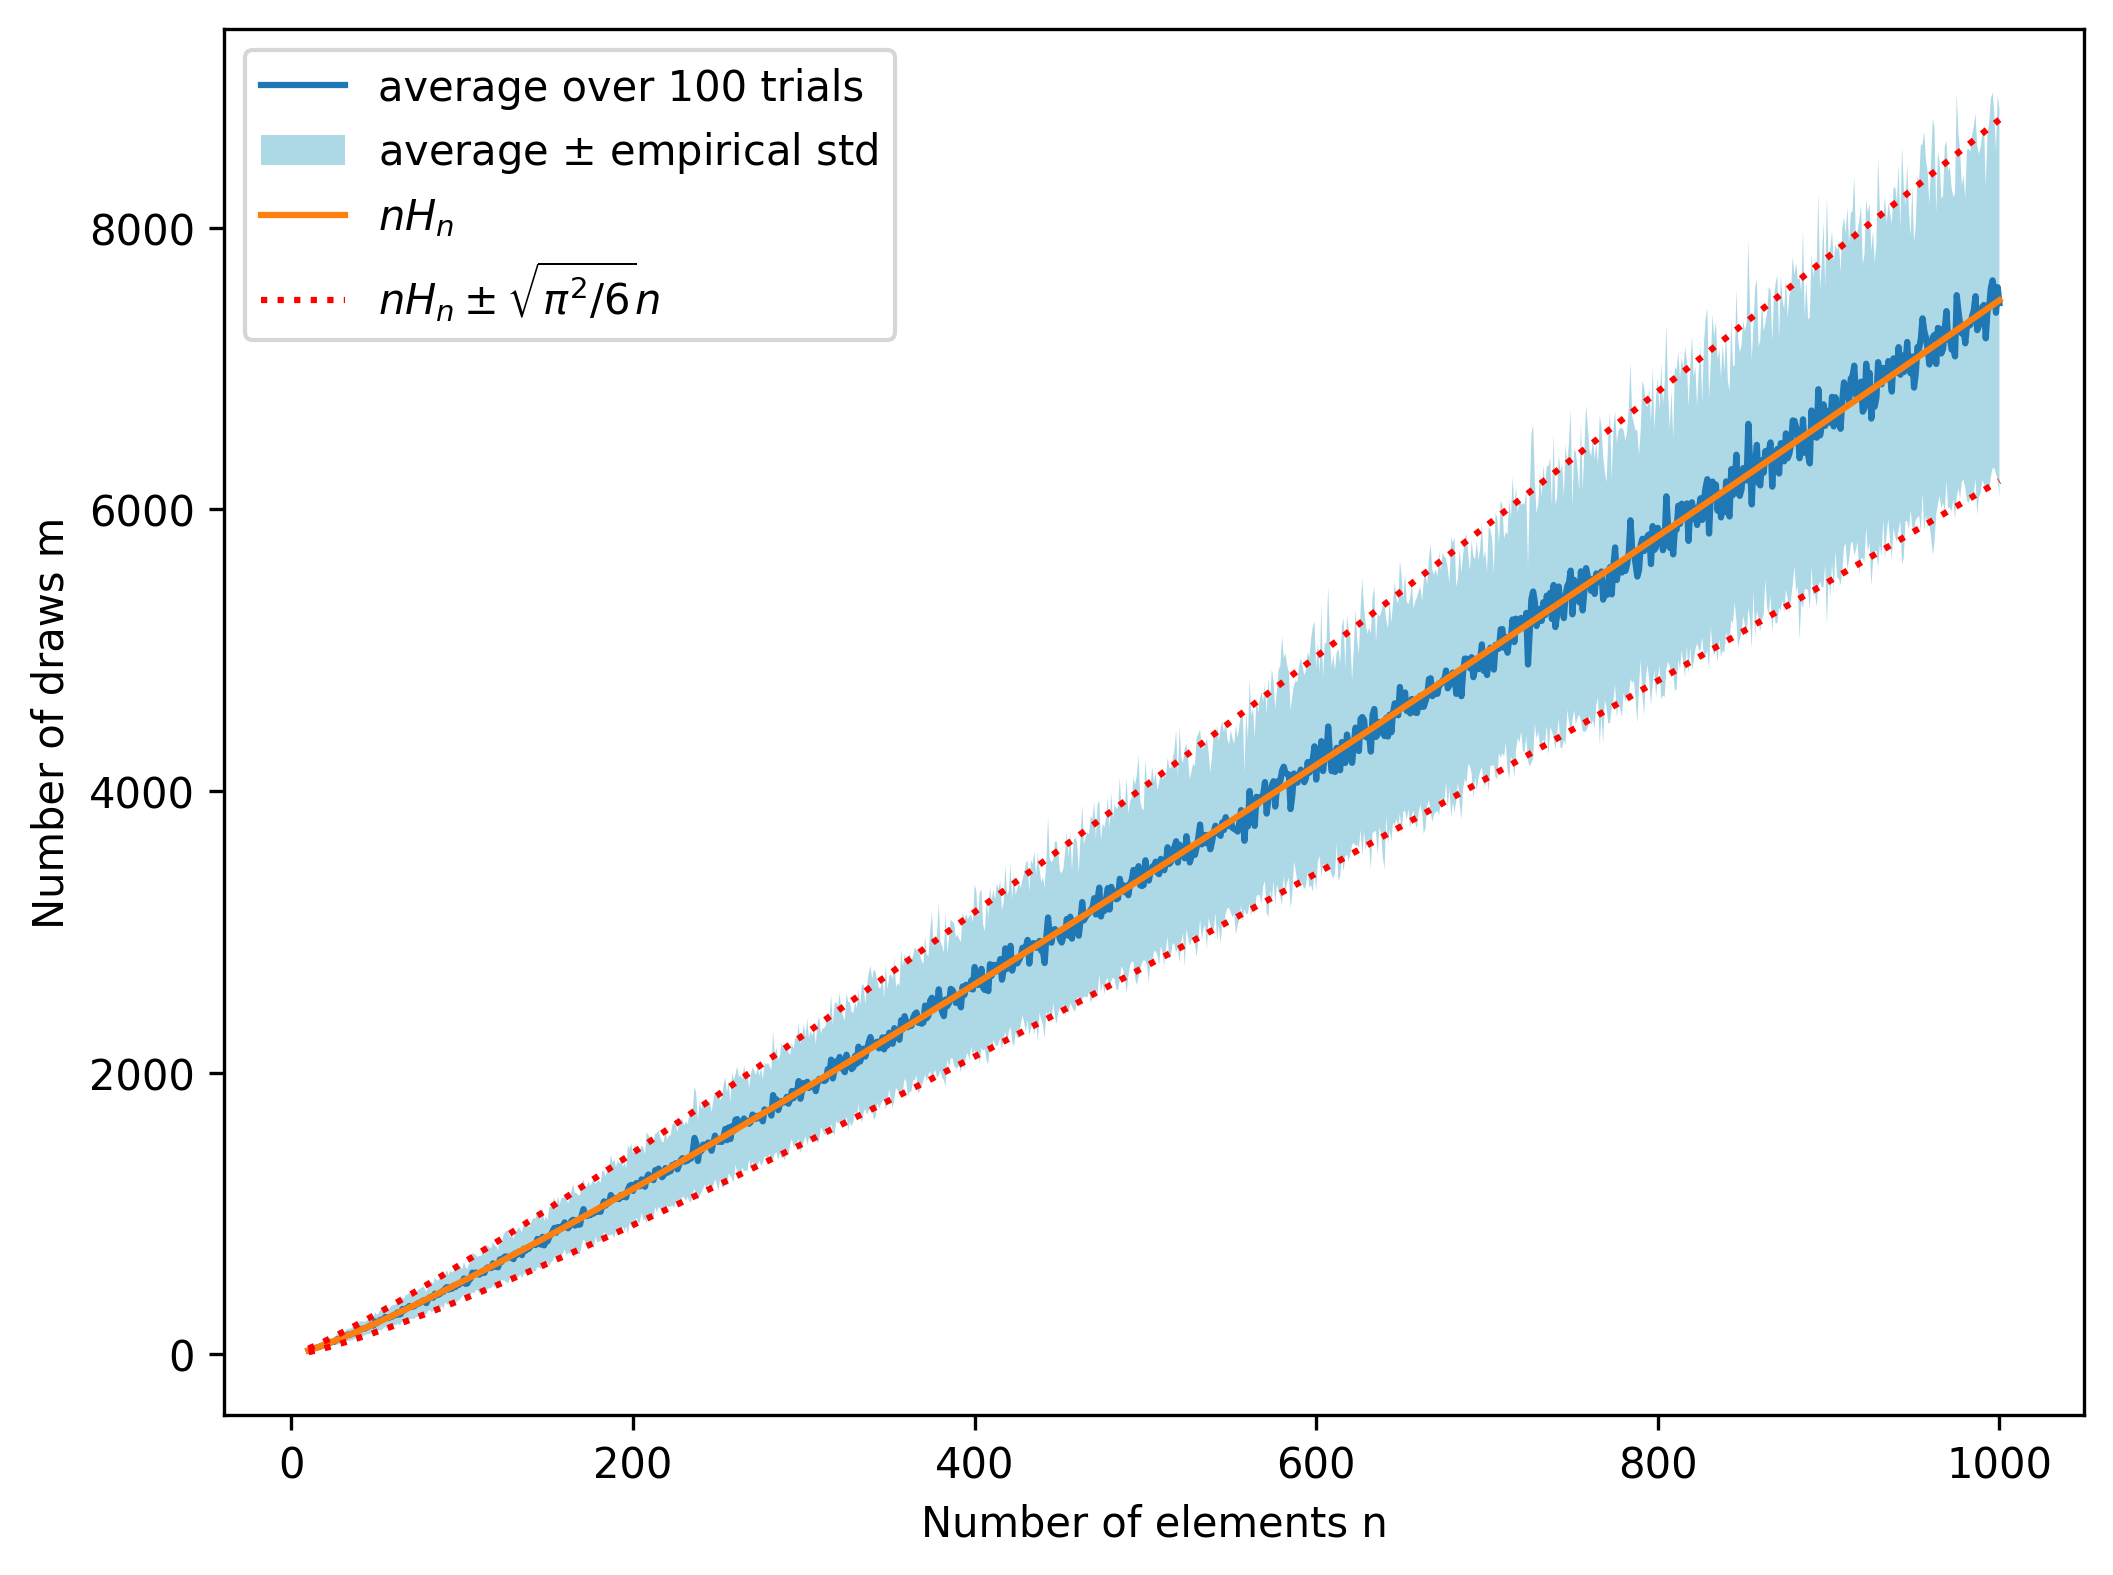
\includegraphics[width=0.9\textwidth]{figures/fig-coverage4.png}
\caption{Average (over 100 trials) of the number of balls thrown until all of the $\nbins$ bins contain at least one ball, as a function of $\nbins$, along with the theoretical value $\nbins H_{\nbins}$ shown in~\cref{theo:coupon:collector:expectation}. The range given by one empirical standard deviation is plotted alongside, as well as the theoretical standard deviation bound obtained.}
\end{figure}

Quite good!

% fun? https://math.stackexchange.com/questions/4051815/intuition-behind-the-coupon-collector-problem-is-there-inclusion-exclusion-prin

\section{Load balancing}
For the last problem considered in this chapter, let us fix $\nballs = \nbins$, and look at how ``balanced'' the bin contents are. In particular, we will be interested in the \emph{maximum load} of the bins:\marginnote{This has applications to, \eg resource allocations, scheduling, etc.}
\begin{framed}
We throw $\nbins$ balls into $\nbins$ bins: what the (expected) number $\orange{L}(\nbins)$ of balls the \emph{fullest} bin will contain?
\end{framed}
Let us denote by $\orange{L}_1,\dots,\orange{L}_{\nbins}$ the number of balls contained in each of the $\nbins$ bins. We have, of course, $\orange{L}_i \leq \nbins$ (number of balls in total) for every $i$. But that's\dots{} quite weak.

It is not hard to see that each bin, separately, follows a Binomial distribution with parameters $\nbins$ and $1/\nbins$\marginnote{Each $\orange{L}_i$ is a $\binomial{\nbins}{1/\nbins}$ random variable: but $\orange{L}_1,\dots,\orange{L}_{\nbins}$ are \emph{not} independent.} and so bin $i$ will have expected load 
\[
\expect{\orange{L}_i} = \nbins\cdot \frac{1}{\nbins} = 1
\]and we also get 
\[
\var[\orange{L}_i] = \nbins\cdot \frac{1}{\nbins}\Paren{1-\frac{1}{\nbins}} \leq 1
\]
This implies, By Chebyshev's inequality, that for each $1\leq i\leq \nbins$, and setting $t \eqdef \sqrt{2\nbins}$,
\[
\probaOf{ \orange{L}_i \geq 1+\sqrt{2\nbins} } \leq \probaOf{ |\orange{L}_i - \expect{\orange{L}_i}| \geq t } \leq \frac{\var[\orange{L}_i]}{t^2} \leq \frac{1}{2\nbins}
\]
and so, by a union bound over the $\nbins$ bins, 
\[
\probaOf{ \max_{1\leq i\leq\nbins}\orange{L}_i \geq 1+\sqrt{2\nbins} } \leq \nbins\cdot \frac{1}{2\nbins} =  \frac{1}{2}
\]
That ``simple'' application of Chebyshev shows the maximum load $\orange{L} = \max_{1\leq i\leq\nbins}$ is $O(\sqrt{\nbins})$ with constant probability. But is it tight? And what does that tell us about $\orange{L}(\nbins)=\expect{\orange{L}}$?\medskip

As in the previous sections, before jumping to conclusions, let's run a simulation.
\begin{lstlisting}
def maxload(n,m):
    loads = np.zeros(n, dtype=int)
    for _ in range(m):
        draw = random.randint(1, n);
        loads[draw-1] += 1
    return np.max(loads)
\end{lstlisting}
\begin{lstlisting}
list_n = np.arange(10, 1001);
experiments_maxload_avg = np.zeros(np.size(list_n));
experiments_maxload_std = np.zeros(np.size(list_n));
for i in range(len(list_n)):
    maxload_trials = [maxload(list_n[i],list_n[i]) for _ in range(100)];
    experiments_maxload_avg[i] = np.mean(maxload_trials);
    experiments_maxload_std[i] = np.std(maxload_trials);
\end{lstlisting}
\begin{figure}[htbp]\centering
    \label{fig:maxload:1}
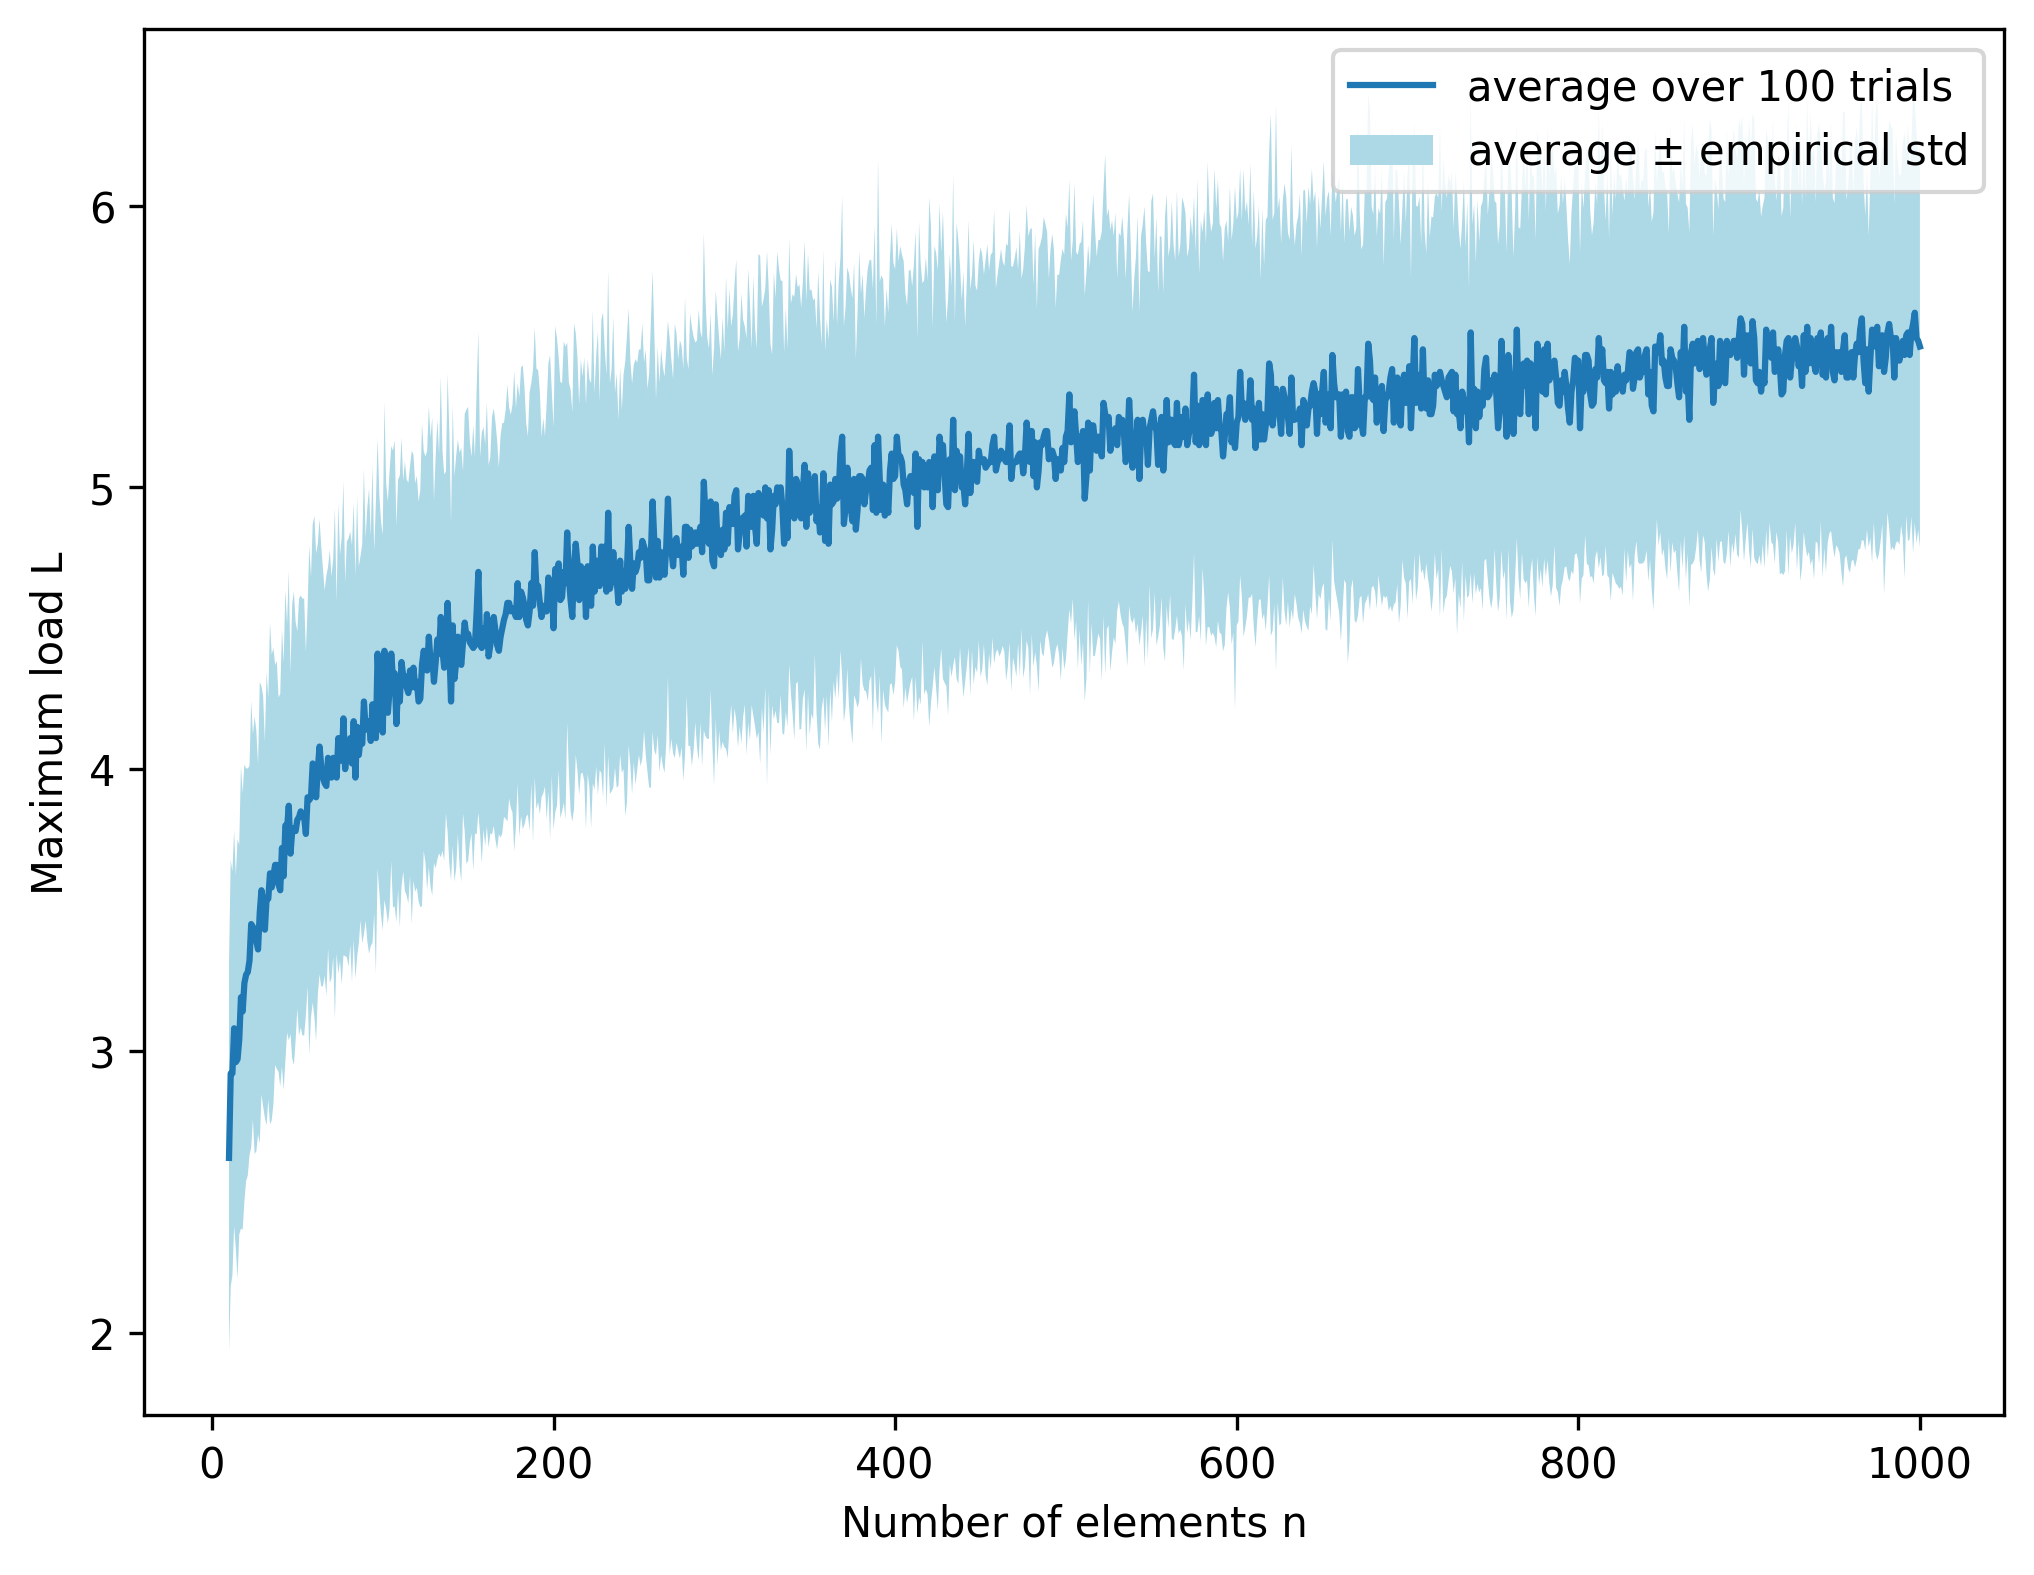
\includegraphics[width=0.9\textwidth]{figures/fig-maxload1.png}
\caption{Average (over 100 trials) of the maximum load when throwing $\nbins$ balls into $\nbins$ bins, as a function of $\nbins$. The range given by one empirical standard deviation is plotted alongside.}
\end{figure}

Looking at the graph (\cref{fig:maxload:1}), we can see how the average maximum load grows with $\nbins$. But what is it, quantitatively? How does $\orange{L}(\nbins)$ behaves?
\begin{itemize}
    \item $\Theta(\log\nbins)$?
    \item $\Theta(\sqrt{\nbins})$?
    \item $\Theta(\nbins)$?
    \item Something else?
\end{itemize}
And \emph{why}?\marginnote{This one will be tough.}\medskip

We will show that, oddly, the answer is ``something else.'' Something quite surprising:
\begin{theorem}
    \label{theo:maxload}
    The expected maximum load $\orange{L}(\nbins)$ when throwing uniformly and independently $\nbins$ balls into $\nbins$ bins grows as
    \[
        \orange{L}(\nbins) = \bigTheta{\frac{\log\nbins}{\log\log\nbins}}\,.
    \]
\end{theorem}
\begin{proof}[Proof of the upper bound of~\cref{theo:maxload}]
Fix any $1\leq i\leq \nbins$, and consider the load in bin $i$. For $0\leq \ell\leq \nbins$, we will give an upper bound on the probability that at least $\ell$ balls fall in this bin: namely, 
\begin{equation}
    \probaOf{\orange{L}_i \geq \ell} 
    \leq \frac{1}{\ell^\ell} 
\end{equation}
To prove this: $\probaOf{\orange{L}_i \geq \ell}$ is the probability that there exists a subset $S\subseteq[\nbins]$ of size at least $\ell$ (a subset of our $\nbins$ balls), and these $|S|$ balls are \emph{exactly} the ones which fell in the $i$-th bin (not a single other): for a fixed $S$, this has probability $\Paren{\frac{1}{\nbins}}^{|S|}\Paren{1-\frac{1}{\nbins}}^{\nbins-|S|}$. We \emph{could} write exactly
\begin{align*}
    \probaOf{\orange{L}_i \geq \ell} 
    &=
    \sum_{\substack{S\subseteq [\nbins]\\ |S| \geq \ell}} \frac{1}{\nbins^{|S|}}\Paren{1-\frac{1}{\nbins}}^{\nbins-|S|} 
    = \sum_{k=\ell}^{\nbins} \sum_{\substack{S\subseteq [\nbins]\\ |S| = k}} \frac{1}{\nbins^{k}}\Paren{1-\frac{1}{\nbins}}^{\nbins-k} \\
    &= \sum_{k=\ell}^{\nbins} \binom{\nbins}{k}\frac{1}{\nbins^{k}}\Paren{1-\frac{1}{\nbins}}^{\nbins-k} %\tag{$\binom{\nbins}{k}$: number of subsets of size $k$}\\
%    &\leq \binom{\nbins}{\ell}\frac{1}{\nbins^{\ell}}\Paren{1-\frac{1}{\nbins}}^{\nbins-\ell}\\
%    &\leq \binom{\nbins}{\ell}\frac{1}{\nbins^{\ell}} 
\end{align*}
the last line recalling that $\binom{\nbins}{k}$ is number of subsets of $[\ns]$ of size $k$, and try to bound that last expression: it is possible, but rather annoying (as binomial coefficients often are), and we do not need to be \emph{that} precise: we just need a good enough upper bound! So we can instead allow ourselves a bit of double-counting: let us simply sum over all subsets $S$ of size \emph{exactly} $\ell$, and focus on the probability that all these $\ell$ balls fall in bin $i$. The other $\ns-\ell$ balls could fall anywhere, including in bin $i$:\footnote{That's the ``we may be double-counting some events'' part.} we don't really care, as long as the upper bound we end up with is not too loose.\marginnote{Exercise: check that $\sum_{k=\ell}^{\nbins} \binom{\nbins}{k}\frac{1}{\nbins^{k}}\Paren{1-\frac{1}{\nbins}}^{\nbins-k} \leq \binom{\nbins}{\ell}\frac{1}{\nbins^{\ell}}$ via a direct computation.}
\begin{align*}
    \probaOf{\orange{L}_i \geq \ell} 
    &\leq
    \sum_{\substack{S\subseteq [\nbins]\\ |S| = \ell}} \probaOf{\text{all }\ell \text{ balls indexed by } S \text{ fall in bin } i} \\
    &=  \sum_{\substack{S\subseteq [\nbins]\\ |S| = \ell}} \left(\frac{1}{\ns}\right)^\ell \\
    &= \binom{\nbins}{\ell}\frac{1}{\nbins^{\ell}} \tag{There are $\binom{\ns}{\ell}$ subsets of size $\ell$}
\end{align*}
From here, we will use this \emph{very} convenient and useful inequality on binomial coefficients:\marginnote{Another life saver.}
\begin{fact}
    \label{fact:binom:coeffs}
    For every $1\leq k\leq n$,
    \[
        \Paren{\frac{n}{k}}^k 
        \leq \binom{n}{k} 
        \leq \Paren{\frac{e n}{k}}^k\,.
    \]
\end{fact}
\noindent This directly leads to the claimed bound
\[
    \probaOf{\orange{L}_i \geq \ell} 
    \leq \Paren{\frac{e \nbins}{\ell}}^{\ell}\frac{1}{\nbins^{\ell}} 
    = \frac{e^\ell}{\ell^\ell}\,.
\]
By a union bound over all $1\leq i\leq \nbins$, we can then conclude that, for every $\ell \geq 1$,
\begin{equation}
    \probaOf{\orange{L} \geq \ell} \leq \sum_{i=1}^{\nbins}\probaOf{\orange{L}_i \geq \ell}
    \leq \frac{\nbins e^\ell}{\ell^\ell}
\end{equation}
This is a very good bound for large $\ell$, but it is quite useless for small $\ell$: for instance, for $\ell=1$, it gives a vacuous bound! Of course, another bound we have is $\probaOf{\orange{L} \geq \ell}  \leq 1$. We will need that, too. Let $\ell(\nbins)$ be the smallest value such that\marginnote{This is the value of $\ell$ starting at which we should switch from using $\probaOf{\orange{L} \geq \ell}  \leq 1$ to using $\probaOf{\orange{L} \geq \ell}  \leq \frac{\nbins e^{\ell}}{\ell^\ell}$, as the latter becomes better.}
\begin{equation}
    \ell(\nbins)^{\ell(\nbins)}e^{-\ell(\ns)} \geq \nbins\,.
\end{equation}
Alright: let us proceed to bounding the expectation of $\orange{L}$. We can write, since $\orange{L}$ is a non-negative integer-valued random variable,\marginnote{Dividing the summation in two parts and using a different bound for both is a standard, handy trick.}
\begin{align}
    L(\nbins) = \expect{\orange{L}} 
    &= \sum_{\ell=1}^\infty \probaOf{\orange{L} \geq \ell} \notag\\
    &= \sum_{\ell=1}^{\ell(\nbins)} \probaOf{\orange{L} \geq \ell} + \sum_{\ell=\ell(\nbins)+1}^\infty \probaOf{\orange{L} \geq \ell} \notag\\
    &\leq \sum_{\ell=1}^{\ell(\nbins)} 1 + \sum_{\ell=\ell(\nbins)+1}^\infty \frac{\nbins e^\ell}{\ell^\ell} \tag{Where the action happens} \notag\\
    &\leq \ell(\nbins) + \sum_{\ell=\ell(\nbins)+1}^\infty \frac{\nbins e^\ell}{\ell(\nbins)^\ell} \notag\\
    &= \ell(\nbins) + \frac{\nbins e^{\ell(\nbins)}}{\ell(\nbins)^{\ell(\nbins)}}\sum_{\ell=\ell(\nbins)+1}^\infty \frac{e^{\ell-\ell(\nbins)}}{\ell(\nbins)^{\ell-\ell(\nbins)}} \notag\\
    &= \ell(\nbins) + \frac{\nbins e^{\ell(\nbins)}}{\ell(\nbins)^{\ell(\nbins)}}\sum_{j=1}^\infty \frac{e^j}{\ell(\nbins)^{j}} \notag\\
    &\leq \ell(\nbins) + \sum_{j=1}^\infty \frac{1}{2^{j}} \tag{as $\frac{\nbins e^{\ell(\nbins)}}{\ell(\nbins)^{\ell(\nbins)}} \leq 1$, and $\ell(\nbins)\geq 2e$} \notag\\
    &= \ell(\nbins) + 1 \label{eq:ub:maxload}
\end{align}
so all that remains to do to conclude is to give an upper bound on $\ell(\nbins)$ itself. This part is not too bad: by definition of $\ell(\nbins)$, we know that
\[
    (\ell(\nbins)-1)^{\ell(\nbins)-1}e^{-(\ell(\nbins)-1))} < \nbins
\]
and taking logarithms, we get
$
(\ell(\nbins)-1)\log (e^{-1}(\ell(\nbins)-1)) < \log \nbins
$. One can ``easily''\marginnote{Exercise: show it.} show that this implies
\[
\ell(\nbins) = \bigTheta{\frac{\log\nbins}{\log\log\nbins}}
\]
which combined with~\eqref{eq:ub:maxload} proves that
$
\boxed{L(\nbins) = \bigO{\frac{\log\nbins}{\log\log\nbins}}}
$.

\paragraph{What about the lower bound?} We will only \emph{sketch} the lower bound in these notes, trying to focus on the key insights. The first insight is that $\orange{L}_1, \dots, \orange{L}_{\nbins}$, which are Binomial r.v.'s with parameters $\nbins$ and $1/\nbins$, are well approximated by a different, ``nicer'' type of of random variable, \emph{Poisson} random variables with parameter $\nbins\cdot 1/\nbins=1$. \marginnote{More generally, 
\[
\boxed{\binomial{n}{\frac{\lambda}{n}} \approx \poisson{\lambda}}
\]
for constant $\lambda>0$. This is very handy!} So we will ``assume'' for convenience\marginnote{This is not an actual proof! But it can be turned into one.} that we can instead consider $\orange{L}'_1, \dots, \orange{L}'_{\nbins} \sim \poisson{1}$. What's more, we will even make the (also not justified! But good for intuition) that these $\orange{L}'_1, \dots, \orange{L}'_{\nbins}$ are independent.

We then can write, since $\expect{\orange{L}} = \sum_{k=1}^\infty \probaOf{\orange{L} \geq k}$, that, for any fixed $\ell\geq 1$ of our choosing,
\begin{align*}
\expect{\orange{L}} &\geq \sum_{k=1}^\ell \probaOf{\orange{L} \geq k} \geq \ell \probaOf{\orange{L} \geq \ell} = 
\ell \probaOf{\exists i,\, \orange{L}_i \geq \ell}
\\
&\approx \ell \probaOf{\exists i,\, \orange{L}'_i \geq \ell}
\geq  \ell \probaOf{\exists i,\, \orange{L}'_i = \ell}
\end{align*}
where the $\approx$ is the first ``sketchy'' Poisson approximation. Using our (unwarranted, sketchy) independence of the $\orange{L}'_i$'s, we can continue by writing\marginnote{If $N\sim\poisson{\lambda}$, then for every non-negative integer $k$
\[
\boxed{\probaOf{N=k} = e^{-\lambda}\frac{\lambda^k}{k!}\,.}
\]}
\begin{align*}
\probaOf{\exists i,\, \orange{L}'_i = \ell}
&= 1-\probaOf{\forall i,\, \orange{L}'_i \neq \ell} \\
&= 1-\Paren{ 1- \frac{e^{-1}}{\ell!} }^{\nbins} \tag{Independence}\\
&\geq 1-e^{-\frac{\nbins}{\ell!}} \tag{using $\ln(1-x)\geq -x$}\\
&\geq 1-e^{-\frac{\nbins}{\ell^\ell}} \tag{using $\ell! \leq \ell^\ell$}\\
\end{align*}
Suitably choosing \[
\ell = \bigTheta{\frac{\log\nbins}{\log\log\nbins}}
\] we get $e^{-\frac{\nbins}{\ell^\ell}} \leq 1/2$, from which $\probaOf{\exists i,\, \orange{L}'_i = \ell} \geq 1/2$. So overall (again, modulo the sketchy bits~--~this is not a full proof), we get
\[
\expect{\orange{L}} \geq \ell \cdot \frac{1}{2} = \bigOmega{\frac{\log\nbins}{\log\log\nbins}}
\]
``showing'' the lower bound.
\end{proof}

\paragraph{Alternative (advanced) proof of the upper bound \advancedstuff} Here is a ``slick'' proof, which seems somewhat magical, but has a couple neat tricks that you will see again or are worth internalizing.\marginnote{Go over it during the tutorials!}

Recall that we want to bound the quantity
\[
\orange{L}(\nbins) = \expect{\max_{1\leq i\leq \nbins} \orange{L}_i}
\]
where the loads $L_1,\dots,L_{\nbins}$ are \emph{not} independent, but all follow a $\operatorname{Binom}(\nbins, 1/\nbins)$ distribution. One can then give an upper bound on $\orange{L}(\nbins)$ as follows.\marginnote{The idea is to replace the $\max$ by a $\sum$ in order to use linearity of expectation~--~but $\max_i \leq \sum_i$ is too lossy, so first we ``exponentiate'' the random variables to mitigate that loss,  as $\max_i \exp \leq \sum_i \exp$ should be ``exponentially less lossy.'' \emph{But} to exponentiate we write $X = \ln \exp X$, which means we now have a $\log$ inside the expectation, and that is not easy to handle: thankfully, $\ln$ is concave, so we can use Jensen's inequality to write $\expect{\ln} \leq \ln\expect{}$. We might also lose something in this step, but that ``Jensen gap'' is typically small for nice, well-concentrated random variables, so\dots{} we can try and hope for the best.}
First, introduce a free parameter $\blue{t}>0$ to be determined later, when we want to optimise the final bound we get.
\begin{align}
    \orange{L}(\nbins) &= \frac{1}{\blue{t}}\cdot \expect{\max_{1\leq i\leq \nbins} \blue{t}\orange{L}_i} \notag\\
    &= \frac{1}{\blue{t}}\cdot \expect{\ln e^{\max_{1\leq i\leq \nbins} \blue{t}\orange{L}_i}} \notag\\
    &\leq \frac{1}{\blue{t}}\cdot \ln\expect{ e^{\max_{1\leq i\leq \nbins} \blue{t}\orange{L}_i}} \tag{Jensen's}\\
    &= \frac{1}{\blue{t}}\cdot \ln\expect{\max_{1\leq i\leq \nbins} e^{\blue{t}\orange{L}_i}} \tag{$\exp{\max_i} = \max_i \exp$}\\
    &\leq \frac{1}{\blue{t}}\cdot \ln\expect{\sum_{1\leq i\leq \nbins} e^{\blue{t}\orange{L}_i}} \tag{$\max_i\leq \sum_i$}\\
    &= \frac{1}{\blue{t}}\cdot \ln \sum_{1\leq i\leq \nbins} \expect{e^{\blue{t}\orange{L}_i}} \tag{Linearity}\\
    &= \frac{1}{\blue{t}}\cdot \ln \nbins \expect{e^{\blue{t}\orange{L}_1}} \label{eq:mgf:maxload}%\\
    %&= \frac{1}{\blue{t}}\Paren{ \ln \nbins + \ln\expect{e^{\blue{t}\orange{L}_1}} }
\end{align}
where the last step used the fact that $L_1,\dots, L_{\nbins}$ all have the same distribution. Now, this quantity $\expect{e^{\blue{t}\orange{L}_1}}$ is called the \emph{moment-generating function} (MGF) of the random variable $\orange{L}_1$, and as a function of $\blue{t}$ it encodes a lot of information about the distribution of $\orange{L}_1$. Thankfully, we do \emph{not} have to compute it: it is standard enough that Wikipedia lists the MGFs for most probability distributions of interest, and in particular for a Binomial random variable $X$ with parameters $n$ and $p$ we have
\begin{equation}
    \expect{e^{tX}} = (1+(e^t-1)p)^n, \qquad t\in\R
\end{equation}
In our case, $p = 1/\nbins$, so we get
\[
    \expect{e^{\blue{t}\orange{L}_1}} 
    = \Paren{1+\frac{e^{\blue{t}}-1}{\nbins}}^{\nbins}
\]
and, using this along with the standard inequality $\ln(1+x) \leq x$ ($x> -1$) in~\eqref{eq:mgf:maxload},\marginnote{This one is a life saver.}
\begin{align}
    \orange{L}(\nbins) 
    &\leq \frac{1}{\blue{t}}\Paren{ \ln \nbins + \ln\expect{e^{\blue{t}\orange{L}_1}} } \notag\\
    &\leq \frac{1}{\blue{t}}\Paren{ \ln \nbins + \nbins\ln\Paren{1+\frac{e^{\blue{t}}-1}{\nbins}} } \notag\\
    &\leq \frac{1}{\blue{t}}\Paren{ \ln \nbins + e^{\blue{t}}-1 } \label{eq:mgf:maxload:freeparam}
\end{align}
We're almost there! We still have our free parameter $\blue{t}>0$, and we get to choose it however we want in order to get the best upper bound possible (we get a valid upper bound no matter which $\blue{t}$ we pick). One option to do so would be to differentiate the RHS of~\eqref{eq:mgf:maxload:freeparam} to find the minimum: this is unfortunately quite unwieldy. A simpler (and most of the time ``good enough''\marginnote{If one does not care too much about the exact constant factors or lower-order terms.} is to observe that
\begin{equation}
\max(a,b) \leq a+b \leq 2\max(a,b), \qquad a,b\geq 0
\end{equation}
and so \emph{minimising a sum of two terms is roughly the same as minimising the maximum.} Here we have two terms: $\ln \nbins$ and $e^{\blue{t}}-1$: one way to make sure the maximum is not too bad is to ``balance it out'', and choose $\blue{t}$ so that the two terms are equal.\marginnote{Useful trick: avoids calculus.} In our case, this means choosing
\begin{equation}
\blue{t} \eqdef \ln\Paren{1+\ln \nbins} = \ln\ln(e\nbins)
\end{equation}
and plugging this choice of $\blue{t}$ in~\eqref{eq:mgf:maxload:freeparam} gives
\begin{equation}
    \label{eq:mgf:maxload:end}
    \orange{L}(\nbins)
    \leq \frac{2\ln \nbins}{\ln\ln(e\nbins)}\,.
\end{equation}
We're done!


\section{Load balancing: the power of two choices}
To conclude, let us mention an even more counter-intuitive result: imagine that instead of throwing $\nbins$ balls uniformly into $\nbins$ bins, each ball instead selects \emph{two} bins uniformly at random, and falls into the \emph{least} full of the two (breaking ties arbitrarily).\marginnote{This looks strange, but has applications to hashing, task allocation, network broadcasting\dots} What becomes the expected maximum load?

As usual, let us first try to get a sense of what is going on via a simulation:
\begin{lstlisting}
def maxload2choices(n,m):
    loads = np.zeros(n, dtype=int)
    for _ in range(m):
        draw1 = random.randint(1, n);
        draw2 = random.randint(1, n);
        if loads[draw2-1] > loads[draw1-1]:
            loads[draw1-1] += 1
        else:
            loads[draw2-1] += 1
    return np.max(loads)
\end{lstlisting}
\begin{lstlisting}
list_n = np.arange(10, 1001);
experiments_maxload2choices_avg = np.zeros(np.size(list_n));
experiments_maxload2choices_std = np.zeros(np.size(list_n));
for i in range(len(list_n)):
    maxload2choices_trials = [maxload2choices(list_n[i],list_n[i]) for _ in range(100)];
    experiments_maxload2choices_avg[i] = np.mean(maxload2choices_trials);
    experiments_maxload2choices_std[i] = np.std(maxload2choices_trials);
\end{lstlisting}
\begin{figure}[htbp]\centering
    \label{fig:maxload:2}
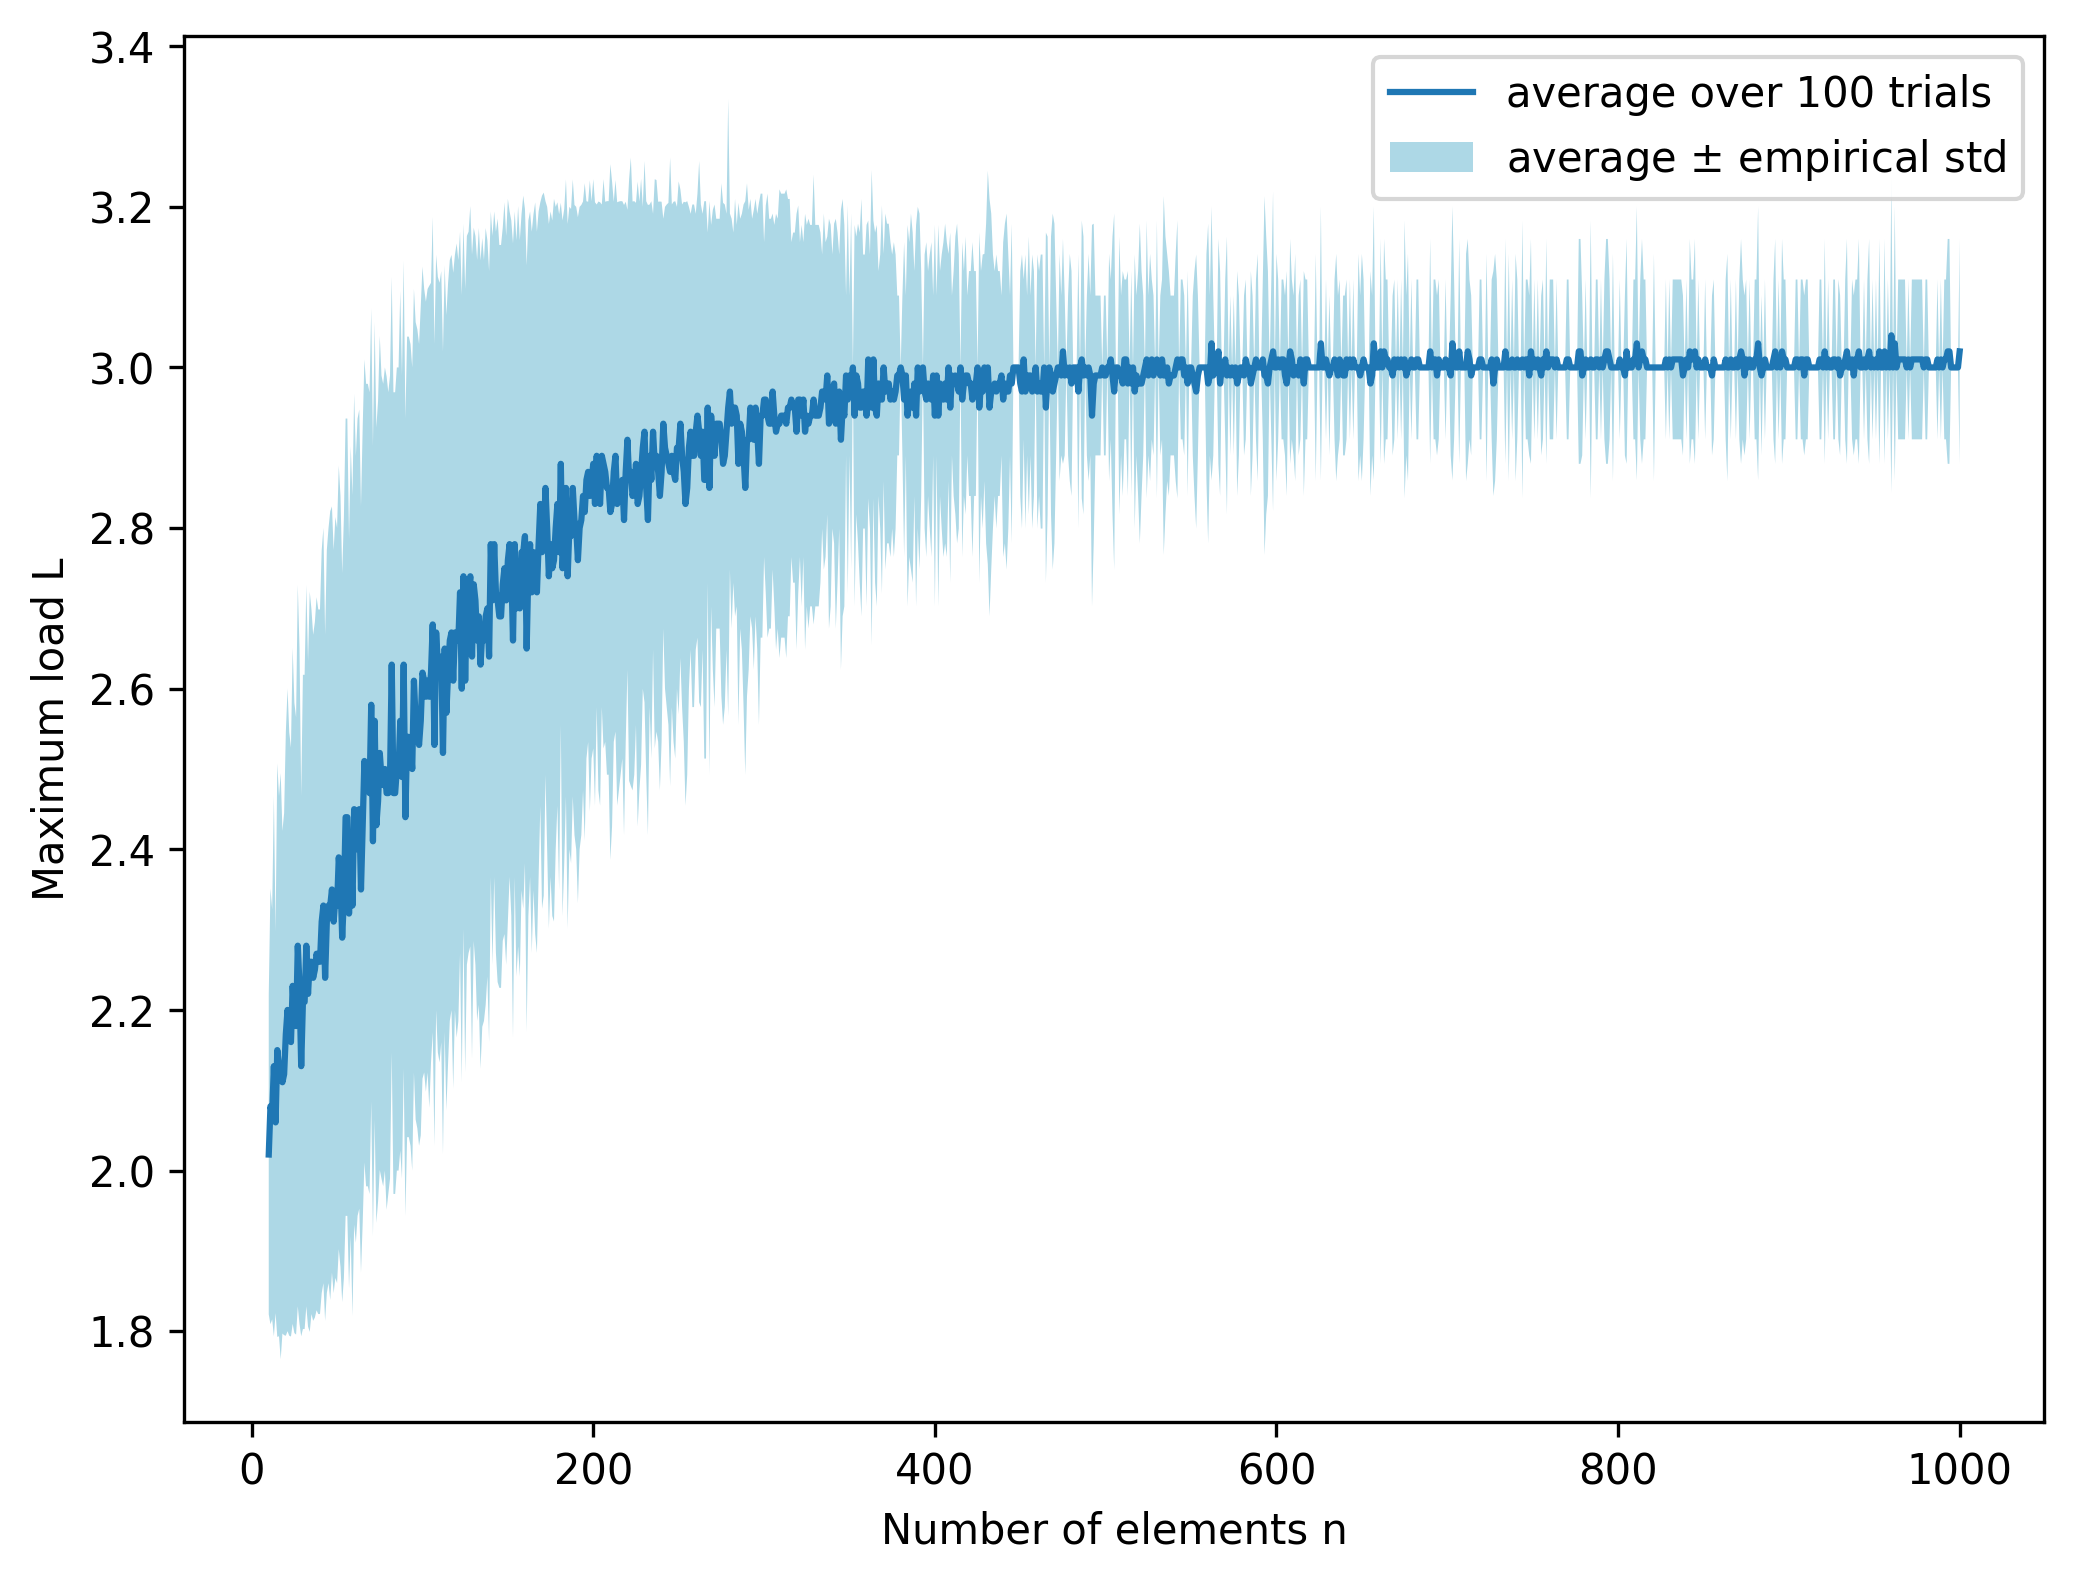
\includegraphics[width=0.9\textwidth]{figures/fig-maxload2choices.png}
\caption{Average (over 100 trials) of the maximum load when throwing $\nbins$ balls into $\nbins$ bins, using the ``best of two bins'' strategy for each bin, as a function of $\nbins$. The range given by one empirical standard deviation is plotted alongside.}
\end{figure}

Looking at the graph (\cref{fig:maxload:2}), we can see that with this ``best of two choices'' the maximum load grows much slower (as a function of $\nbins$) than in the previous setting (\cref{fig:maxload:1}). But how much slower? %How does $\orange{\hat{L}}(\nbins)$ behaves?
\begin{itemize}
    \item $\Theta(\sqrt{\log\nbins})$?
    \item $\bigTheta{\frac{\log\nbins}{(\log\log\nbins)^2}}$?
    \item $\Theta(\log\log\nbins)$?
    \item Something else?
\end{itemize}
\marginnote{\TODO{} in class: Visualization of the maximum load as $\nballs$ increases, i.e., as more balls are thrown (same with power of two choices).}

\noindent Amazingly, this simple ``power of two choices'' brings the expected maximum load from $\bigTheta{\frac{\log\nbins}{\log\log\nbins}}$ to something \emph{exponentially smaller}:
\begin{theorem}
    \label{theo:maxload:twochoices}
    The expected maximum load $\orange{\hat{L}}(\nbins)$ when throwing independently $\nbins$ balls into $\nbins$ bins using the ``best of two choices'' strategy above grows as
    \[
        \orange{\hat{L}}(\nbins) = \log\log\nbins + O(1)\,.
    \]
\end{theorem}
\noindent(We will not prove this theorem in the lecture.)